% Options for packages loaded elsewhere
\PassOptionsToPackage{unicode}{hyperref}
\PassOptionsToPackage{hyphens}{url}
\PassOptionsToPackage{dvipsnames,svgnames*,x11names*}{xcolor}
%
\documentclass[
]{article}
\usepackage{lmodern}
\usepackage{amssymb,amsmath}
\usepackage{ifxetex,ifluatex}
\ifnum 0\ifxetex 1\fi\ifluatex 1\fi=0 % if pdftex
  \usepackage[T1]{fontenc}
  \usepackage[utf8]{inputenc}
  \usepackage{textcomp} % provide euro and other symbols
\else % if luatex or xetex
  \usepackage{unicode-math}
  \defaultfontfeatures{Scale=MatchLowercase}
  \defaultfontfeatures[\rmfamily]{Ligatures=TeX,Scale=1}
\fi
% Use upquote if available, for straight quotes in verbatim environments
\IfFileExists{upquote.sty}{\usepackage{upquote}}{}
\IfFileExists{microtype.sty}{% use microtype if available
  \usepackage[]{microtype}
  \UseMicrotypeSet[protrusion]{basicmath} % disable protrusion for tt fonts
}{}
\makeatletter
\@ifundefined{KOMAClassName}{% if non-KOMA class
  \IfFileExists{parskip.sty}{%
    \usepackage{parskip}
  }{% else
    \setlength{\parindent}{0pt}
    \setlength{\parskip}{6pt plus 2pt minus 1pt}}
}{% if KOMA class
  \KOMAoptions{parskip=half}}
\makeatother
\usepackage{xcolor}
\IfFileExists{xurl.sty}{\usepackage{xurl}}{} % add URL line breaks if available
\IfFileExists{bookmark.sty}{\usepackage{bookmark}}{\usepackage{hyperref}}
\hypersetup{
  pdftitle={Final Project},
  pdfauthor={STAT 420, Summer 2020, Mandalorians},
  colorlinks=true,
  linkcolor=Maroon,
  filecolor=Maroon,
  citecolor=Blue,
  urlcolor=cyan,
  pdfcreator={LaTeX via pandoc}}
\urlstyle{same} % disable monospaced font for URLs
\usepackage[margin=1in]{geometry}
\usepackage{color}
\usepackage{fancyvrb}
\newcommand{\VerbBar}{|}
\newcommand{\VERB}{\Verb[commandchars=\\\{\}]}
\DefineVerbatimEnvironment{Highlighting}{Verbatim}{commandchars=\\\{\}}
% Add ',fontsize=\small' for more characters per line
\usepackage{framed}
\definecolor{shadecolor}{RGB}{248,248,248}
\newenvironment{Shaded}{\begin{snugshade}}{\end{snugshade}}
\newcommand{\AlertTok}[1]{\textcolor[rgb]{0.94,0.16,0.16}{#1}}
\newcommand{\AnnotationTok}[1]{\textcolor[rgb]{0.56,0.35,0.01}{\textbf{\textit{#1}}}}
\newcommand{\AttributeTok}[1]{\textcolor[rgb]{0.77,0.63,0.00}{#1}}
\newcommand{\BaseNTok}[1]{\textcolor[rgb]{0.00,0.00,0.81}{#1}}
\newcommand{\BuiltInTok}[1]{#1}
\newcommand{\CharTok}[1]{\textcolor[rgb]{0.31,0.60,0.02}{#1}}
\newcommand{\CommentTok}[1]{\textcolor[rgb]{0.56,0.35,0.01}{\textit{#1}}}
\newcommand{\CommentVarTok}[1]{\textcolor[rgb]{0.56,0.35,0.01}{\textbf{\textit{#1}}}}
\newcommand{\ConstantTok}[1]{\textcolor[rgb]{0.00,0.00,0.00}{#1}}
\newcommand{\ControlFlowTok}[1]{\textcolor[rgb]{0.13,0.29,0.53}{\textbf{#1}}}
\newcommand{\DataTypeTok}[1]{\textcolor[rgb]{0.13,0.29,0.53}{#1}}
\newcommand{\DecValTok}[1]{\textcolor[rgb]{0.00,0.00,0.81}{#1}}
\newcommand{\DocumentationTok}[1]{\textcolor[rgb]{0.56,0.35,0.01}{\textbf{\textit{#1}}}}
\newcommand{\ErrorTok}[1]{\textcolor[rgb]{0.64,0.00,0.00}{\textbf{#1}}}
\newcommand{\ExtensionTok}[1]{#1}
\newcommand{\FloatTok}[1]{\textcolor[rgb]{0.00,0.00,0.81}{#1}}
\newcommand{\FunctionTok}[1]{\textcolor[rgb]{0.00,0.00,0.00}{#1}}
\newcommand{\ImportTok}[1]{#1}
\newcommand{\InformationTok}[1]{\textcolor[rgb]{0.56,0.35,0.01}{\textbf{\textit{#1}}}}
\newcommand{\KeywordTok}[1]{\textcolor[rgb]{0.13,0.29,0.53}{\textbf{#1}}}
\newcommand{\NormalTok}[1]{#1}
\newcommand{\OperatorTok}[1]{\textcolor[rgb]{0.81,0.36,0.00}{\textbf{#1}}}
\newcommand{\OtherTok}[1]{\textcolor[rgb]{0.56,0.35,0.01}{#1}}
\newcommand{\PreprocessorTok}[1]{\textcolor[rgb]{0.56,0.35,0.01}{\textit{#1}}}
\newcommand{\RegionMarkerTok}[1]{#1}
\newcommand{\SpecialCharTok}[1]{\textcolor[rgb]{0.00,0.00,0.00}{#1}}
\newcommand{\SpecialStringTok}[1]{\textcolor[rgb]{0.31,0.60,0.02}{#1}}
\newcommand{\StringTok}[1]{\textcolor[rgb]{0.31,0.60,0.02}{#1}}
\newcommand{\VariableTok}[1]{\textcolor[rgb]{0.00,0.00,0.00}{#1}}
\newcommand{\VerbatimStringTok}[1]{\textcolor[rgb]{0.31,0.60,0.02}{#1}}
\newcommand{\WarningTok}[1]{\textcolor[rgb]{0.56,0.35,0.01}{\textbf{\textit{#1}}}}
\usepackage{longtable,booktabs}
% Correct order of tables after \paragraph or \subparagraph
\usepackage{etoolbox}
\makeatletter
\patchcmd\longtable{\par}{\if@noskipsec\mbox{}\fi\par}{}{}
\makeatother
% Allow footnotes in longtable head/foot
\IfFileExists{footnotehyper.sty}{\usepackage{footnotehyper}}{\usepackage{footnote}}
\makesavenoteenv{longtable}
\usepackage{graphicx,grffile}
\makeatletter
\def\maxwidth{\ifdim\Gin@nat@width>\linewidth\linewidth\else\Gin@nat@width\fi}
\def\maxheight{\ifdim\Gin@nat@height>\textheight\textheight\else\Gin@nat@height\fi}
\makeatother
% Scale images if necessary, so that they will not overflow the page
% margins by default, and it is still possible to overwrite the defaults
% using explicit options in \includegraphics[width, height, ...]{}
\setkeys{Gin}{width=\maxwidth,height=\maxheight,keepaspectratio}
% Set default figure placement to htbp
\makeatletter
\def\fps@figure{htbp}
\makeatother
\setlength{\emergencystretch}{3em} % prevent overfull lines
\providecommand{\tightlist}{%
  \setlength{\itemsep}{0pt}\setlength{\parskip}{0pt}}
\setcounter{secnumdepth}{5}

\title{Final Project}
\author{STAT 420, Summer 2020, Mandalorians}
\date{}

\begin{document}
\maketitle

{
\hypersetup{linkcolor=}
\setcounter{tocdepth}{2}
\tableofcontents
}
\DeclareUnicodeCharacter{00A0}{~}

\begin{center}\rule{0.5\linewidth}{0.5pt}\end{center}

\hypertarget{introduction}{%
\section{Introduction}\label{introduction}}

We have a housing dataset. We have pulled this dataset as part of a kaggle challenge. We have the train and test data as separate files. Since this is a challenge, we dont have the predicted values for the test dataset.

Our job is to predict house prices, given 80 predictors.

We can see the structure of the dataset below

\begin{Shaded}
\begin{Highlighting}[]
\NormalTok{df1 <-}\KeywordTok{read.csv}\NormalTok{(}\StringTok{"train.csv"}\NormalTok{,}\DataTypeTok{as.is =} \OtherTok{FALSE}\NormalTok{ )}

\KeywordTok{str}\NormalTok{(df1)}
\end{Highlighting}
\end{Shaded}

\begin{verbatim}
## 'data.frame':    1460 obs. of  81 variables:
##  $ Id           : int  1 2 3 4 5 6 7 8 9 10 ...
##  $ MSSubClass   : int  60 20 60 70 60 50 20 60 50 190 ...
##  $ MSZoning     : Factor w/ 5 levels "C (all)","FV",..: 4 4 4 4 4 4 4 4 5 4 ...
##  $ LotFrontage  : int  65 80 68 60 84 85 75 NA 51 50 ...
##  $ LotArea      : int  8450 9600 11250 9550 14260 14115 10084 10382 6120 7420 ...
##  $ Street       : Factor w/ 2 levels "Grvl","Pave": 2 2 2 2 2 2 2 2 2 2 ...
##  $ Alley        : Factor w/ 2 levels "Grvl","Pave": NA NA NA NA NA NA NA NA NA NA ...
##  $ LotShape     : Factor w/ 4 levels "IR1","IR2","IR3",..: 4 4 1 1 1 1 4 1 4 4 ...
##  $ LandContour  : Factor w/ 4 levels "Bnk","HLS","Low",..: 4 4 4 4 4 4 4 4 4 4 ...
##  $ Utilities    : Factor w/ 2 levels "AllPub","NoSeWa": 1 1 1 1 1 1 1 1 1 1 ...
##  $ LotConfig    : Factor w/ 5 levels "Corner","CulDSac",..: 5 3 5 1 3 5 5 1 5 1 ...
##  $ LandSlope    : Factor w/ 3 levels "Gtl","Mod","Sev": 1 1 1 1 1 1 1 1 1 1 ...
##  $ Neighborhood : Factor w/ 25 levels "Blmngtn","Blueste",..: 6 25 6 7 14 12 21 17 18 4 ...
##  $ Condition1   : Factor w/ 9 levels "Artery","Feedr",..: 3 2 3 3 3 3 3 5 1 1 ...
##  $ Condition2   : Factor w/ 8 levels "Artery","Feedr",..: 3 3 3 3 3 3 3 3 3 1 ...
##  $ BldgType     : Factor w/ 5 levels "1Fam","2fmCon",..: 1 1 1 1 1 1 1 1 1 2 ...
##  $ HouseStyle   : Factor w/ 8 levels "1.5Fin","1.5Unf",..: 6 3 6 6 6 1 3 6 1 2 ...
##  $ OverallQual  : int  7 6 7 7 8 5 8 7 7 5 ...
##  $ OverallCond  : int  5 8 5 5 5 5 5 6 5 6 ...
##  $ YearBuilt    : int  2003 1976 2001 1915 2000 1993 2004 1973 1931 1939 ...
##  $ YearRemodAdd : int  2003 1976 2002 1970 2000 1995 2005 1973 1950 1950 ...
##  $ RoofStyle    : Factor w/ 6 levels "Flat","Gable",..: 2 2 2 2 2 2 2 2 2 2 ...
##  $ RoofMatl     : Factor w/ 8 levels "ClyTile","CompShg",..: 2 2 2 2 2 2 2 2 2 2 ...
##  $ Exterior1st  : Factor w/ 15 levels "AsbShng","AsphShn",..: 13 9 13 14 13 13 13 7 4 9 ...
##  $ Exterior2nd  : Factor w/ 16 levels "AsbShng","AsphShn",..: 14 9 14 16 14 14 14 7 16 9 ...
##  $ MasVnrType   : Factor w/ 4 levels "BrkCmn","BrkFace",..: 2 3 2 3 2 3 4 4 3 3 ...
##  $ MasVnrArea   : int  196 0 162 0 350 0 186 240 0 0 ...
##  $ ExterQual    : Factor w/ 4 levels "Ex","Fa","Gd",..: 3 4 3 4 3 4 3 4 4 4 ...
##  $ ExterCond    : Factor w/ 5 levels "Ex","Fa","Gd",..: 5 5 5 5 5 5 5 5 5 5 ...
##  $ Foundation   : Factor w/ 6 levels "BrkTil","CBlock",..: 3 2 3 1 3 6 3 2 1 1 ...
##  $ BsmtQual     : Factor w/ 4 levels "Ex","Fa","Gd",..: 3 3 3 4 3 3 1 3 4 4 ...
##  $ BsmtCond     : Factor w/ 4 levels "Fa","Gd","Po",..: 4 4 4 2 4 4 4 4 4 4 ...
##  $ BsmtExposure : Factor w/ 4 levels "Av","Gd","Mn",..: 4 2 3 4 1 4 1 3 4 4 ...
##  $ BsmtFinType1 : Factor w/ 6 levels "ALQ","BLQ","GLQ",..: 3 1 3 1 3 3 3 1 6 3 ...
##  $ BsmtFinSF1   : int  706 978 486 216 655 732 1369 859 0 851 ...
##  $ BsmtFinType2 : Factor w/ 6 levels "ALQ","BLQ","GLQ",..: 6 6 6 6 6 6 6 2 6 6 ...
##  $ BsmtFinSF2   : int  0 0 0 0 0 0 0 32 0 0 ...
##  $ BsmtUnfSF    : int  150 284 434 540 490 64 317 216 952 140 ...
##  $ TotalBsmtSF  : int  856 1262 920 756 1145 796 1686 1107 952 991 ...
##  $ Heating      : Factor w/ 6 levels "Floor","GasA",..: 2 2 2 2 2 2 2 2 2 2 ...
##  $ HeatingQC    : Factor w/ 5 levels "Ex","Fa","Gd",..: 1 1 1 3 1 1 1 1 3 1 ...
##  $ CentralAir   : Factor w/ 2 levels "N","Y": 2 2 2 2 2 2 2 2 2 2 ...
##  $ Electrical   : Factor w/ 5 levels "FuseA","FuseF",..: 5 5 5 5 5 5 5 5 2 5 ...
##  $ X1stFlrSF    : int  856 1262 920 961 1145 796 1694 1107 1022 1077 ...
##  $ X2ndFlrSF    : int  854 0 866 756 1053 566 0 983 752 0 ...
##  $ LowQualFinSF : int  0 0 0 0 0 0 0 0 0 0 ...
##  $ GrLivArea    : int  1710 1262 1786 1717 2198 1362 1694 2090 1774 1077 ...
##  $ BsmtFullBath : int  1 0 1 1 1 1 1 1 0 1 ...
##  $ BsmtHalfBath : int  0 1 0 0 0 0 0 0 0 0 ...
##  $ FullBath     : int  2 2 2 1 2 1 2 2 2 1 ...
##  $ HalfBath     : int  1 0 1 0 1 1 0 1 0 0 ...
##  $ BedroomAbvGr : int  3 3 3 3 4 1 3 3 2 2 ...
##  $ KitchenAbvGr : int  1 1 1 1 1 1 1 1 2 2 ...
##  $ KitchenQual  : Factor w/ 4 levels "Ex","Fa","Gd",..: 3 4 3 3 3 4 3 4 4 4 ...
##  $ TotRmsAbvGrd : int  8 6 6 7 9 5 7 7 8 5 ...
##  $ Functional   : Factor w/ 7 levels "Maj1","Maj2",..: 7 7 7 7 7 7 7 7 3 7 ...
##  $ Fireplaces   : int  0 1 1 1 1 0 1 2 2 2 ...
##  $ FireplaceQu  : Factor w/ 5 levels "Ex","Fa","Gd",..: NA 5 5 3 5 NA 3 5 5 5 ...
##  $ GarageType   : Factor w/ 6 levels "2Types","Attchd",..: 2 2 2 6 2 2 2 2 6 2 ...
##  $ GarageYrBlt  : int  2003 1976 2001 1998 2000 1993 2004 1973 1931 1939 ...
##  $ GarageFinish : Factor w/ 3 levels "Fin","RFn","Unf": 2 2 2 3 2 3 2 2 3 2 ...
##  $ GarageCars   : int  2 2 2 3 3 2 2 2 2 1 ...
##  $ GarageArea   : int  548 460 608 642 836 480 636 484 468 205 ...
##  $ GarageQual   : Factor w/ 5 levels "Ex","Fa","Gd",..: 5 5 5 5 5 5 5 5 2 3 ...
##  $ GarageCond   : Factor w/ 5 levels "Ex","Fa","Gd",..: 5 5 5 5 5 5 5 5 5 5 ...
##  $ PavedDrive   : Factor w/ 3 levels "N","P","Y": 3 3 3 3 3 3 3 3 3 3 ...
##  $ WoodDeckSF   : int  0 298 0 0 192 40 255 235 90 0 ...
##  $ OpenPorchSF  : int  61 0 42 35 84 30 57 204 0 4 ...
##  $ EnclosedPorch: int  0 0 0 272 0 0 0 228 205 0 ...
##  $ X3SsnPorch   : int  0 0 0 0 0 320 0 0 0 0 ...
##  $ ScreenPorch  : int  0 0 0 0 0 0 0 0 0 0 ...
##  $ PoolArea     : int  0 0 0 0 0 0 0 0 0 0 ...
##  $ PoolQC       : Factor w/ 3 levels "Ex","Fa","Gd": NA NA NA NA NA NA NA NA NA NA ...
##  $ Fence        : Factor w/ 4 levels "GdPrv","GdWo",..: NA NA NA NA NA 3 NA NA NA NA ...
##  $ MiscFeature  : Factor w/ 4 levels "Gar2","Othr",..: NA NA NA NA NA 3 NA 3 NA NA ...
##  $ MiscVal      : int  0 0 0 0 0 700 0 350 0 0 ...
##  $ MoSold       : int  2 5 9 2 12 10 8 11 4 1 ...
##  $ YrSold       : int  2008 2007 2008 2006 2008 2009 2007 2009 2008 2008 ...
##  $ SaleType     : Factor w/ 9 levels "COD","Con","ConLD",..: 9 9 9 9 9 9 9 9 9 9 ...
##  $ SaleCondition: Factor w/ 6 levels "Abnorml","AdjLand",..: 5 5 5 1 5 5 5 5 1 5 ...
##  $ SalePrice    : int  208500 181500 223500 140000 250000 143000 307000 200000 129900 118000 ...
\end{verbatim}

\hypertarget{method}{%
\section{Method}\label{method}}

\hypertarget{investigations---1}{%
\subsection{Investigations - 1}\label{investigations---1}}

Now we investigate the dataset to see what actions we need to take with the dataset before creating a model

Since the output is very long, we use echo=FALSE, but as a sample, we show the output below for the first 5 rows

\begin{Shaded}
\begin{Highlighting}[]
\NormalTok{Hmisc}\OperatorTok{::}\KeywordTok{html}\NormalTok{(Hmisc}\OperatorTok{::}\KeywordTok{describe}\NormalTok{(df1[,}\DecValTok{1}\OperatorTok{:}\DecValTok{5}\NormalTok{]), }\DataTypeTok{where=}\KeywordTok{c}\NormalTok{(}\StringTok{'cwd'}\NormalTok{, }\StringTok{'tmp'}\NormalTok{))}
\end{Highlighting}
\end{Shaded}

{df1{[}, 1:5{]} 5 Variables   1460 Observations}

{Id}

{lowest~: 1 2 3 4 5 , highest: 1456 1457 1458 1459 1460}

{MSSubClass}

n

missing

distinct

Info

Mean

Gmd

.05

.10

.25

.50

.75

.90

.95

1460

0

15

0.94

56.9

43.19

20

20

20

50

70

120

160

{lowest~: 20 30 40 45 50 , highest: 90 120 160 180 190}

{MSZoning}

n

missing

distinct

1460

0

5

{lowest~: C (all) FV RH RL RM , highest: C (all) FV RH RL RM }

{LotFrontage}

n

missing

distinct

Info

Mean

Gmd

.05

.10

.25

.50

.75

.90

.95

1201

259

110

0.998

70.05

24.61

34

44

59

69

80

96

107

{lowest~: 21 24 30 32 33 , highest: 160 168 174 182 313}

{LotArea}

n

missing

distinct

Info

Mean

Gmd

.05

.10

.25

.50

.75

.90

.95

1460

0

1073

1

10517

5718

3312

5000

7554

9478

11602

14382

17401

{lowest~: 1300 1477 1491 1526 1533 , highest: 70761 115149 159000 164660 215245}

\hypertarget{interim-cleanup---1}{%
\subsection{Interim Cleanup - 1}\label{interim-cleanup---1}}

We have 80 predictors in the dataset. That tells us that we really arent short of predictors.

Based on the above dataset description (showing only first 5 for brevity) we draw the following conclusions

\textbf{Remove these columns}

\begin{itemize}
\tightlist
\item
  Remove Id column since it is not a predictor and is simply a running id
\item
  Alley - has 1369 missing values and only 91 observations with values.
\item
  Street - Only 6 elements or 0.4\% data elements have Street as Grvl, rest are all Pave. 6 is too few data elements to make a prediction
\item
  LotFrontage has 259 missing values. This is about 18\% of total observations. If we were short of predictors we would not delete it. Since there a lot of predictors that convey space of the house, we will delete this column
\item
  Utilities - Only 1 value has NoSeWa and the rest are all AllPub. Since only 1 element isnt enough for creating a model
\item
  Condition2 - remove since 99\% are Norm while the remaining 1\% are distributed across 7 other values. This implies that the other 7 values dont have enough data to make a useful prediction
\item
  RoofMatl - 98.2\% is CompShg and the remaining 1.8\% is spread across 7 values and the remaining 7 values dont have enough data to make a prediction
\item
  X3SsnPorch - 98.4\% is value 0, and the remaining 1.6\% is spread across 19 types. Each of these has only 1 or 2 observtions hence not enough data for prediction
\item
  PoolArea - 99.5\% has value 0 and the remaining .5\% is apread across 7 factors, implying not enough data in each type to make a model
\item
  PoolQC - since only 7 observations have non missing values
\item
  MiscFeature, MiscVal - since only 54 and 52 observations respectively have values
\item
  FirePlaceQu - has 690 values missing which is approximately 47\% of total predictors. Since we are not short of number of predictors, and this one has half the values missing, we will delete this predictor
\item
  Fence - 1179 values missing.
\end{itemize}

\textbf{Other Observations}

\begin{itemize}
\tightlist
\item
  MasVnrType and MasVnrArea - has 8 missing values
\item
  BsmtQual, BsmtCond, BsmtExposure, BsmtFinType1, BsmtFinType2 - each have 37 or 38 missing values
\item
  Electrical = has 1 value missing
\item
  GarageType, GarageYrBlt, GarageFinish, GarageQual, GarageCond - has 81 values missing
\end{itemize}

Based on the above analysis we remove the ones that we want to remove and store the column names for the ones with missing values in a vector to be used later if necessary

\begin{Shaded}
\begin{Highlighting}[]
\NormalTok{remove_cols <-}\StringTok{ }\KeywordTok{c}\NormalTok{(}\StringTok{"Id"}\NormalTok{, }\StringTok{"Alley"}\NormalTok{, }\StringTok{"Street"}\NormalTok{, }\StringTok{"LotFrontage"}\NormalTok{, }\StringTok{"Utilities"}\NormalTok{, }\StringTok{"Condition2"}\NormalTok{, }\StringTok{"RoofMatl"}\NormalTok{, }\StringTok{"X3SsnPorch"}\NormalTok{, }\StringTok{"PoolArea"}\NormalTok{, }\StringTok{"PoolQC"}\NormalTok{, }\StringTok{"MiscFeature"}\NormalTok{, }\StringTok{"MiscVal"}\NormalTok{, }\StringTok{"FireplaceQu"}\NormalTok{, }\StringTok{"Fence"}\NormalTok{)}

\NormalTok{col_with_missing_values <-}\StringTok{ }\KeywordTok{c}\NormalTok{(}\StringTok{"MasVnrType"}\NormalTok{, }\StringTok{"MasVnrArea"}\NormalTok{, }\StringTok{"BsmtQual"}\NormalTok{, }\StringTok{"BsmtCond"}\NormalTok{, }\StringTok{"BsmtExposure"}\NormalTok{, }\StringTok{"BsmtFinType1"}\NormalTok{, }\StringTok{"BsmtFinType2"}\NormalTok{, }\StringTok{"Electrical"}\NormalTok{, }\StringTok{"GarageType"}\NormalTok{, }\StringTok{"GarageYrBlt"}\NormalTok{, }\StringTok{"GarageFinish"}\NormalTok{, }\StringTok{"GarageQual"}\NormalTok{, }\StringTok{"GarageCond"}\NormalTok{)}

\NormalTok{keep_cols <-}\StringTok{ }\KeywordTok{colnames}\NormalTok{(df1)[}\OperatorTok{!}\NormalTok{(}\KeywordTok{colnames}\NormalTok{(df1) }\OperatorTok\StringTok{ }\NormalTok{remove_cols)]}

\NormalTok{df_cols_removed <-}\StringTok{ }\KeywordTok{subset}\NormalTok{(df1, }\DataTypeTok{select =} \KeywordTok{as.vector}\NormalTok{(}\KeywordTok{eval}\NormalTok{(keep_cols)))}
\end{Highlighting}
\end{Shaded}

\hypertarget{investigation---2---correlation}{%
\subsection{Investigation - 2 - Correlation}\label{investigation---2---correlation}}

Now, to identify columns that have high correlations. We define high correlation as great than 70\% correlation.

In order to identify correlation we first create a dataframe that has only numeric predictors

\begin{Shaded}
\begin{Highlighting}[]
\NormalTok{df_only_numeric <-}\StringTok{ }\NormalTok{df_cols_removed[,}\KeywordTok{sapply}\NormalTok{(df_cols_removed, is.numeric)]}
\end{Highlighting}
\end{Shaded}

Now we identify the correlation in numeric predictors. We mark all correlations less than .75 as NA, so that we can easily identify highly corelated features

For breivity of the resport, we only show the head of the corellation matrix, while we had looked at the entire matrix to come to our conclusions below

\begin{Shaded}
\begin{Highlighting}[]
\NormalTok{cor_relation =}\StringTok{ }\KeywordTok{cor}\NormalTok{(df_only_numeric, }\DataTypeTok{use =} \StringTok{"complete.obs"}\NormalTok{)}
\NormalTok{cor_relation[}\KeywordTok{abs}\NormalTok{(cor_relation) }\OperatorTok{<}\StringTok{ }\FloatTok{0.75}\NormalTok{] <-}\StringTok{ }\OtherTok{NA}
\KeywordTok{head}\NormalTok{(cor_relation)}
\end{Highlighting}
\end{Shaded}

\begin{verbatim}
##              MSSubClass LotArea OverallQual OverallCond YearBuilt YearRemodAdd
## MSSubClass            1      NA          NA          NA        NA           NA
## LotArea              NA       1          NA          NA        NA           NA
## OverallQual          NA      NA           1          NA        NA           NA
## OverallCond          NA      NA          NA           1        NA           NA
## YearBuilt            NA      NA          NA          NA         1           NA
## YearRemodAdd         NA      NA          NA          NA        NA            1
##              MasVnrArea BsmtFinSF1 BsmtFinSF2 BsmtUnfSF TotalBsmtSF X1stFlrSF
## MSSubClass           NA         NA         NA        NA          NA        NA
## LotArea              NA         NA         NA        NA          NA        NA
## OverallQual          NA         NA         NA        NA          NA        NA
## OverallCond          NA         NA         NA        NA          NA        NA
## YearBuilt            NA         NA         NA        NA          NA        NA
## YearRemodAdd         NA         NA         NA        NA          NA        NA
##              X2ndFlrSF LowQualFinSF GrLivArea BsmtFullBath BsmtHalfBath
## MSSubClass          NA           NA        NA           NA           NA
## LotArea             NA           NA        NA           NA           NA
## OverallQual         NA           NA        NA           NA           NA
## OverallCond         NA           NA        NA           NA           NA
## YearBuilt           NA           NA        NA           NA           NA
## YearRemodAdd        NA           NA        NA           NA           NA
##              FullBath HalfBath BedroomAbvGr KitchenAbvGr TotRmsAbvGrd
## MSSubClass         NA       NA           NA           NA           NA
## LotArea            NA       NA           NA           NA           NA
## OverallQual        NA       NA           NA           NA           NA
## OverallCond        NA       NA           NA           NA           NA
## YearBuilt          NA       NA           NA           NA           NA
## YearRemodAdd       NA       NA           NA           NA           NA
##              Fireplaces GarageYrBlt GarageCars GarageArea WoodDeckSF
## MSSubClass           NA          NA         NA         NA         NA
## LotArea              NA          NA         NA         NA         NA
## OverallQual          NA          NA         NA         NA         NA
## OverallCond          NA          NA         NA         NA         NA
## YearBuilt            NA   0.8246693         NA         NA         NA
## YearRemodAdd         NA          NA         NA         NA         NA
##              OpenPorchSF EnclosedPorch ScreenPorch MoSold YrSold SalePrice
## MSSubClass            NA            NA          NA     NA     NA        NA
## LotArea               NA            NA          NA     NA     NA        NA
## OverallQual           NA            NA          NA     NA     NA 0.7862117
## OverallCond           NA            NA          NA     NA     NA        NA
## YearBuilt             NA            NA          NA     NA     NA        NA
## YearRemodAdd          NA            NA          NA     NA     NA        NA
\end{verbatim}

\hypertarget{interim-cleanup---2}{%
\subsection{Interim Cleanup - 2}\label{interim-cleanup---2}}

Based on the above correlation matrix, we make the below observations

\textbf{Remove the following predictors}

\begin{itemize}
\tightlist
\item
  YearBuilt and GarageYrBlt has .82 correlation coefficient. This makes sense since the Garage will be built in the same year as the house, with a few exceptions. We also reason that the price will be more tied to how old the house is. Since YearBuilt of house will be a more useful predictor, we will remove GarageYrBlt
\item
  X1stFlrSF and TotalBsmtSF has a .82 correlation. This is obvious since the size of teh 1st floor will be very similar to size of basement. We can also reason that the price will be more correlated to the price of the 1st floor. Hence we will remove TotalBsmtSF
\item
  GarageArea and GarageCars have a .83 correlation. Intutively we can see that both of these are related. Hence we remove GarageCars
\item
  GrLivArea and TotRmsAbvGrd has a correlation of .82. We see that number of Bedrooms and kitchens and batrooms are already captured separately. Hence we remove TotRmsAbvGrd
\end{itemize}

\textbf{Make a note of these}
* OverallQual has a .78 correlation with SalePrice. Given that, we should make sure OverallQual is part of the model

\begin{Shaded}
\begin{Highlighting}[]
\NormalTok{remove_cols2 <-}\StringTok{ }\KeywordTok{c}\NormalTok{(}\StringTok{"GarageYrBlt"}\NormalTok{, }\StringTok{"TotalBsmtSF"}\NormalTok{, }\StringTok{"GarageCars"}\NormalTok{, }\StringTok{"TotRmsAbvGrd"}\NormalTok{)}

\NormalTok{keep_cols2 <-}\StringTok{ }\KeywordTok{colnames}\NormalTok{(df_cols_removed)[}\OperatorTok{!}\NormalTok{(}\KeywordTok{colnames}\NormalTok{(df_cols_removed) }\OperatorTok\StringTok{ }\NormalTok{remove_cols2)]}

\NormalTok{df_cols_removed <-}\StringTok{ }\KeywordTok{subset}\NormalTok{(df_cols_removed, }\DataTypeTok{select =} \KeywordTok{as.vector}\NormalTok{(}\KeywordTok{eval}\NormalTok{(keep_cols2)))}

\KeywordTok{ncol}\NormalTok{(df_cols_removed)}
\end{Highlighting}
\end{Shaded}

\begin{verbatim}
## [1] 63
\end{verbatim}

We see that now we are left with 63 columns compared to the 81 that we started with.

We know that step wont work with missing values. Hence we will need to remove those.

\begin{Shaded}
\begin{Highlighting}[]
\NormalTok{df_cols_removed <-}\StringTok{ }\KeywordTok{na.omit}\NormalTok{(df_cols_removed)}
\KeywordTok{nrow}\NormalTok{(df_cols_removed)}
\end{Highlighting}
\end{Shaded}

\begin{verbatim}
## [1] 1338
\end{verbatim}

We started with 1460 observations and 81 columns and after our initial cleanup we end up with 1338 observations and 63 columns

\hypertarget{transformation-identification}{%
\subsection{Transformation identification}\label{transformation-identification}}

\hypertarget{pairs-plot}{%
\subsubsection{Pairs plot}\label{pairs-plot}}

Now, before we begin modeling, we look at the pairs plots to see if any of the parameters are an obvious choice for transformations

For the purpose of being able to see the plots clearly, we do two things for the visual of the pair plot

\begin{enumerate}
\def\labelenumi{\arabic{enumi})}
\tightlist
\item
  We only look at numeric columns
\item
  We filter out the columns that have 25 or less discrete values, since they will probably not be candidates for transformations
\end{enumerate}

We wont save this intermim dataset. It is only created to be able to see the distribution across many predictors clearly

\begin{Shaded}
\begin{Highlighting}[]
\NormalTok{df_only_numeric <-}\StringTok{ }\NormalTok{df_cols_removed[,}\KeywordTok{sapply}\NormalTok{(df_cols_removed, is.numeric)]}
\NormalTok{remove_for_plot <-}\StringTok{ }\KeywordTok{c}\NormalTok{()}
\NormalTok{j=}\DecValTok{1}
\ControlFlowTok{for}\NormalTok{(i }\ControlFlowTok{in} \KeywordTok{colnames}\NormalTok{(df_only_numeric))\{}
\NormalTok{  k <-}\StringTok{ }\KeywordTok{length}\NormalTok{(}\KeywordTok{unique}\NormalTok{(df_only_numeric[,i])}\OperatorTok{<}\DecValTok{20}\NormalTok{)}
  \ControlFlowTok{if}\NormalTok{(k}\OperatorTok{<}\DecValTok{20}\NormalTok{)\{}
\NormalTok{    remove_for_plot[j] <-}\StringTok{ }\NormalTok{i}
\NormalTok{    j <-}\StringTok{ }\NormalTok{j}\OperatorTok{+}\DecValTok{1}
\NormalTok{  \}}
\NormalTok{\}}

\NormalTok{keep_for_plot <-}\StringTok{ }\KeywordTok{colnames}\NormalTok{(df_only_numeric)[}\OperatorTok{!}\NormalTok{(}\KeywordTok{colnames}\NormalTok{(df_only_numeric) }\OperatorTok\StringTok{ }\NormalTok{remove_for_plot)]}

\NormalTok{df_cols_removed_for_plot <-}\StringTok{ }\KeywordTok{subset}\NormalTok{(df_only_numeric, }\DataTypeTok{select =} \KeywordTok{as.vector}\NormalTok{(}\KeywordTok{eval}\NormalTok{(keep_for_plot)))}
\end{Highlighting}
\end{Shaded}

\begin{Shaded}
\begin{Highlighting}[]
\CommentTok{#pairs(df_only_numeric)}
\KeywordTok{ggpairs}\NormalTok{( df_cols_removed_for_plot, ggplot2}\OperatorTok{::}\KeywordTok{aes}\NormalTok{(}\DataTypeTok{color=}\KeywordTok{I}\NormalTok{(}\StringTok{"navyblue"}\NormalTok{)), }\DataTypeTok{title =} \StringTok{"ggpairs plot to see correlation and distribution"}\NormalTok{, }\DataTypeTok{lower =} \KeywordTok{list}\NormalTok{(}\DataTypeTok{continuous =} \KeywordTok{wrap}\NormalTok{(}\StringTok{"smooth"}\NormalTok{)), }\DataTypeTok{axisLabels =} \StringTok{"show"}\NormalTok{, }\DataTypeTok{switch =} \StringTok{"both"}\NormalTok{)}
\end{Highlighting}
\end{Shaded}

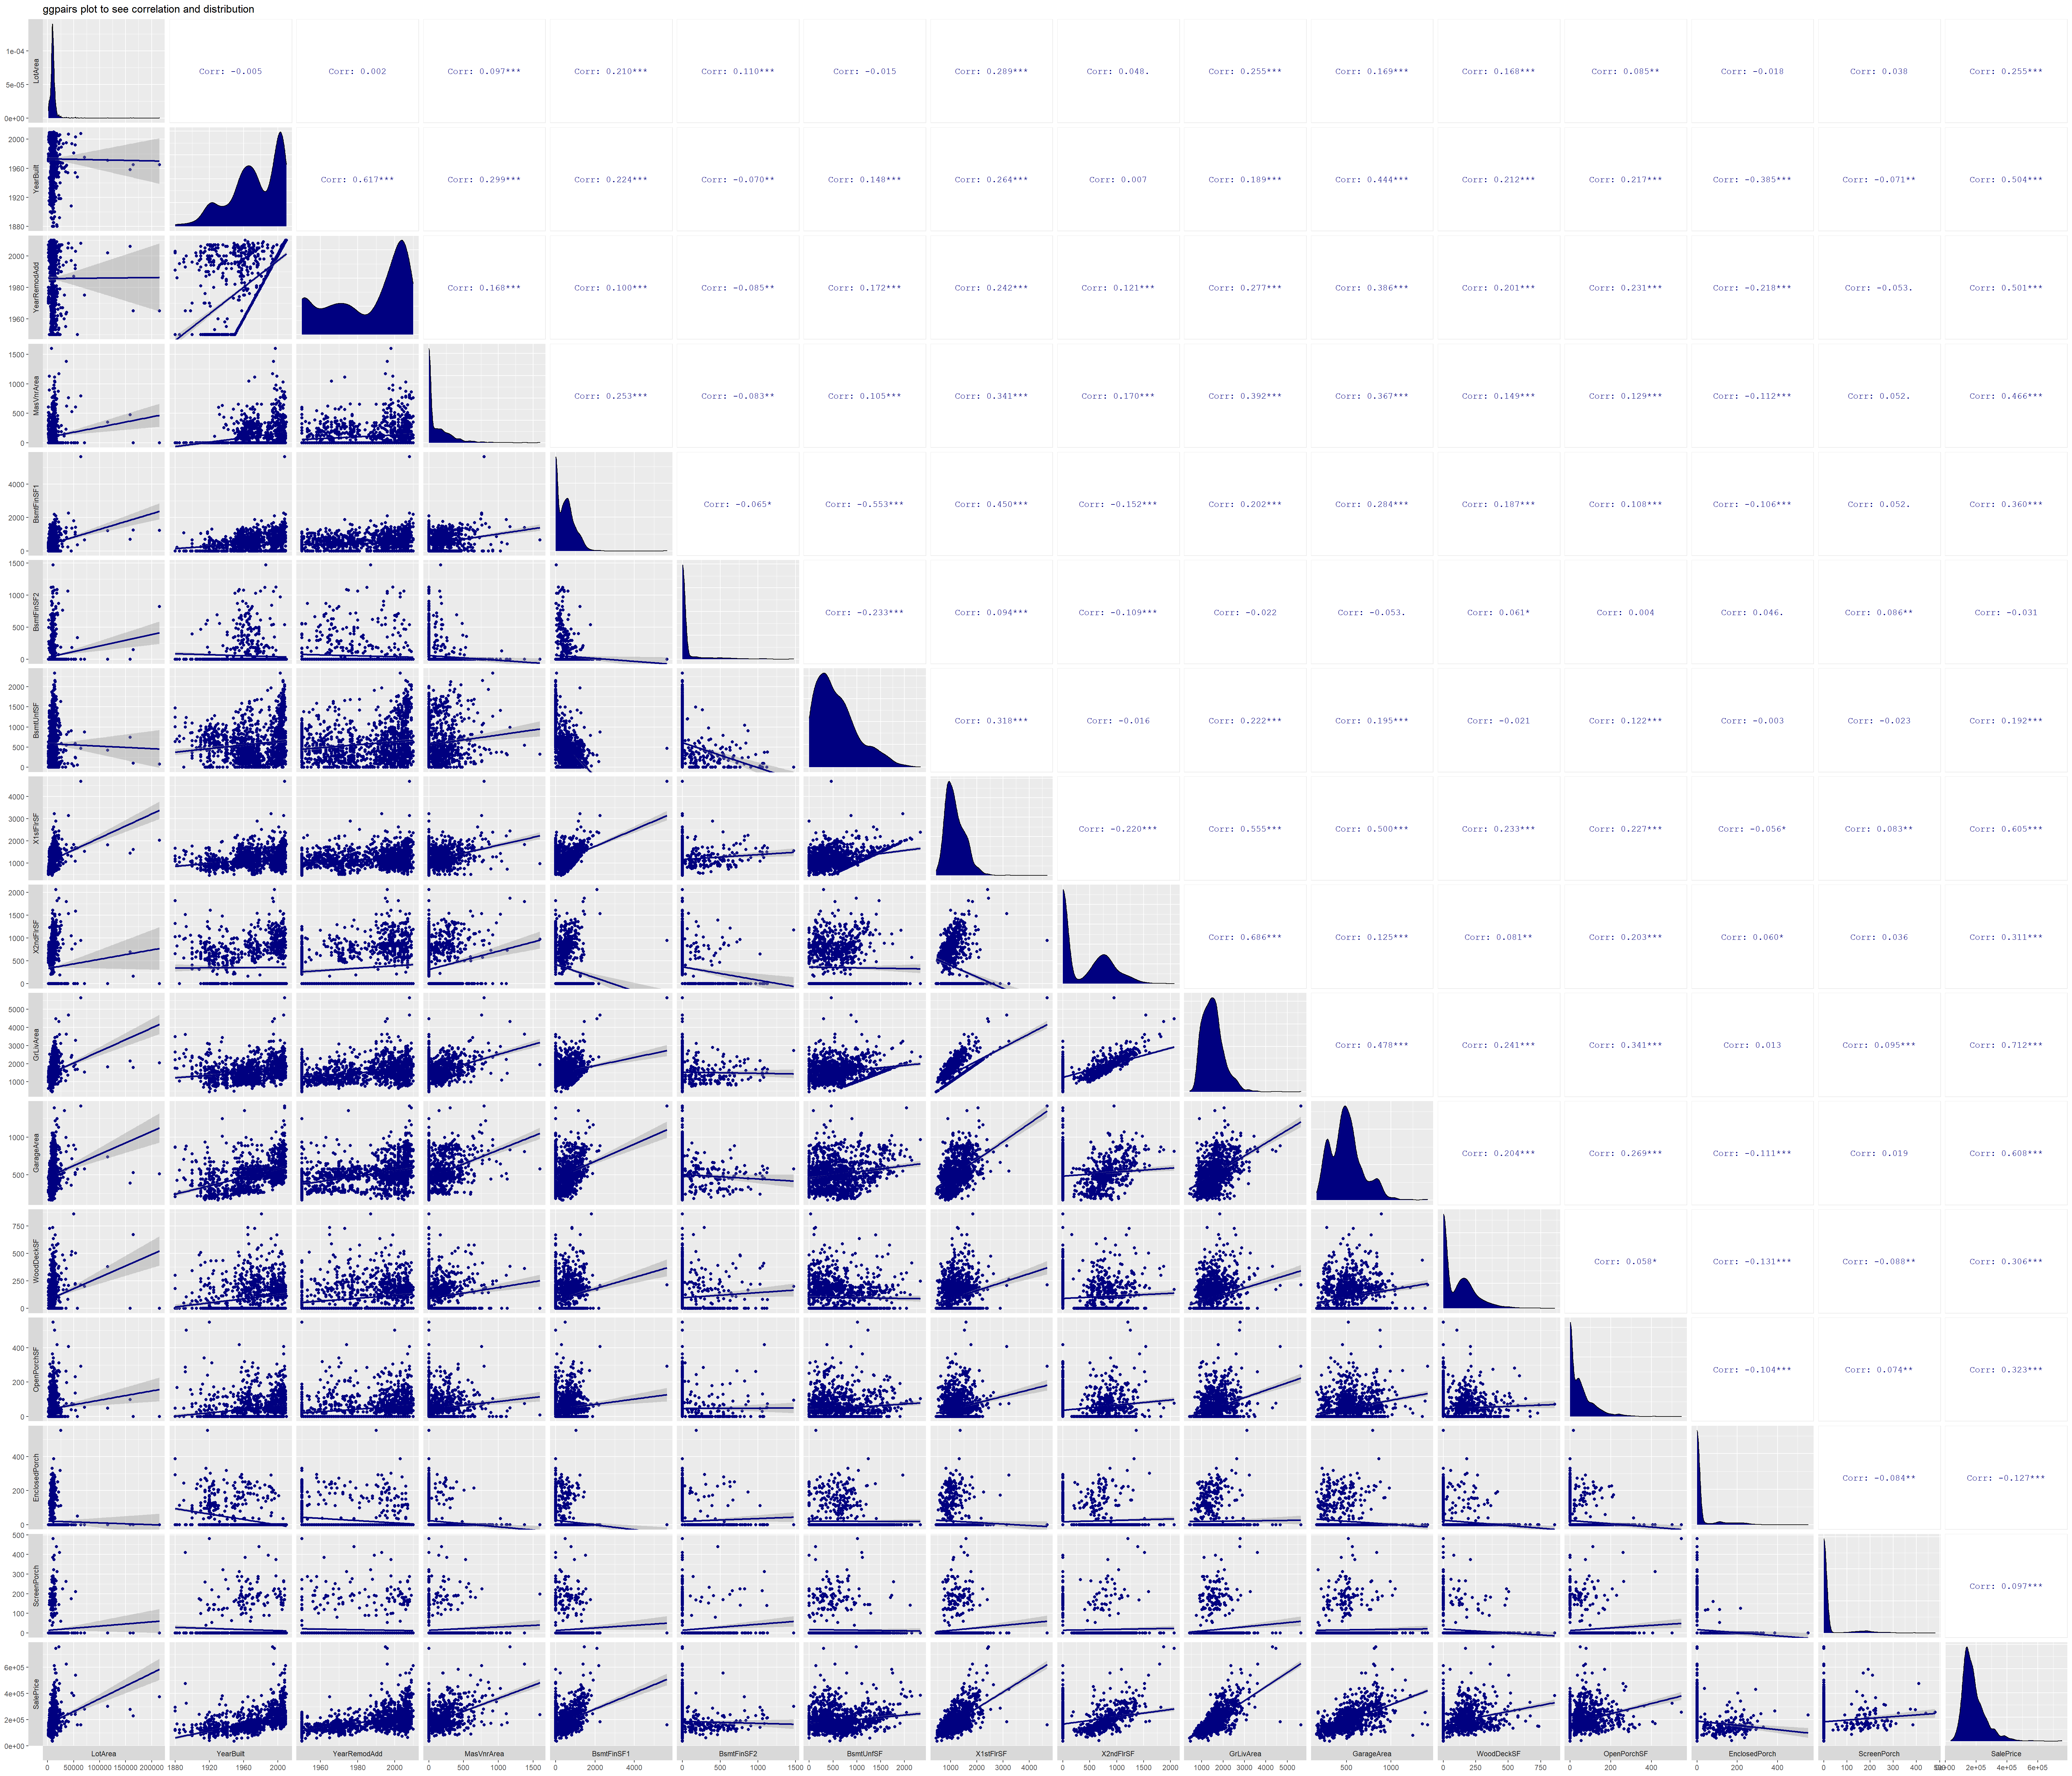
\includegraphics{Final-Project_files/figure-latex/unnamed-chunk-11-1.pdf}

We make the following observations from the plot

** Potential for transformations **

\begin{itemize}
\tightlist
\item
  LotArea
\item
  MasVnrArea
\item
  BsmtFinSF1
\item
  BsmtFinSF2
\item
  X1stFlrSF
\item
  GrLivArea
\item
  GarageArea
\item
  WoodDeckSF
\item
  OpenPorchSF
\item
  EnclosedPorch
\item
  YearBuilt
\item
  YearRemodAdd
\item
  SalePrice
\end{itemize}

\begin{Shaded}
\begin{Highlighting}[]
\NormalTok{diagnostics <-}\StringTok{ }\ControlFlowTok{function}\NormalTok{(}\DataTypeTok{model =}\NormalTok{ fit_}\DecValTok{1}\NormalTok{, }\DataTypeTok{pcol =} \StringTok{'dodgerblue'}\NormalTok{, }\DataTypeTok{lcol =} \StringTok{'red'}\NormalTok{, }\DataTypeTok{alpha =} \FloatTok{.05}\NormalTok{, }\DataTypeTok{plotit =} \OtherTok{TRUE}\NormalTok{, }\DataTypeTok{testit =} \OtherTok{TRUE}\NormalTok{)\{}
  
  \ControlFlowTok{if}\NormalTok{(plotit }\OperatorTok{==}\StringTok{ }\OtherTok{TRUE}\NormalTok{)\{}
\NormalTok{    g1 <-}\StringTok{ }\KeywordTok{ggplot}\NormalTok{(}\DataTypeTok{data =}\NormalTok{ model, }\KeywordTok{aes}\NormalTok{(}\DataTypeTok{sample=}\NormalTok{.resid)) }\OperatorTok{+}\StringTok{ }
\StringTok{      }\KeywordTok{stat_qq}\NormalTok{(}\DataTypeTok{color=}\KeywordTok{I}\NormalTok{(pcol)) }\OperatorTok{+}\StringTok{ }\KeywordTok{stat_qq_line}\NormalTok{(}\DataTypeTok{color =} \KeywordTok{I}\NormalTok{(lcol)) }\OperatorTok{+}
\StringTok{      }\KeywordTok{ggtitle}\NormalTok{(}\StringTok{"Normal QQ Plot"}\NormalTok{) }\OperatorTok{+}\StringTok{  }\KeywordTok{theme_light}\NormalTok{() }
    
\NormalTok{    g2 <-}\StringTok{ }\KeywordTok{ggplot}\NormalTok{(}\DataTypeTok{data =}\NormalTok{ model, }\KeywordTok{aes}\NormalTok{(}\DataTypeTok{x =} \KeywordTok{fitted}\NormalTok{(model), }\DataTypeTok{y =} \KeywordTok{resid}\NormalTok{(model))) }\OperatorTok{+}
\StringTok{      }\KeywordTok{geom_point}\NormalTok{(}\DataTypeTok{color=}\KeywordTok{I}\NormalTok{(pcol)) }\OperatorTok{+}\StringTok{ }\KeywordTok{geom_hline}\NormalTok{(}\DataTypeTok{yintercept=}\DecValTok{0}\NormalTok{, }\DataTypeTok{color =} \KeywordTok{I}\NormalTok{(lcol)) }\OperatorTok{+}
\StringTok{      }\KeywordTok{xlab}\NormalTok{(}\StringTok{"Fitted"}\NormalTok{) }\OperatorTok{+}\StringTok{ }\KeywordTok{ylab}\NormalTok{(}\StringTok{"Residuals"}\NormalTok{) }\OperatorTok{+}\StringTok{ }\KeywordTok{ggtitle}\NormalTok{(}\StringTok{"Residuals vs Fitted Plot"}\NormalTok{) }\OperatorTok{+}\StringTok{ }\KeywordTok{theme_light}\NormalTok{() }
    
    \KeywordTok{grid.arrange}\NormalTok{(g1, g2, }\DataTypeTok{ncol=}\DecValTok{2}\NormalTok{)}
\NormalTok{  \}}
  
  \ControlFlowTok{if}\NormalTok{(testit }\OperatorTok{==}\StringTok{ }\OtherTok{TRUE}\NormalTok{)\{}
\NormalTok{    shapiro_Normalcy_test_result <-}\StringTok{ }\KeywordTok{shapiro.test}\NormalTok{(}\KeywordTok{resid}\NormalTok{(model))}\OperatorTok{$}\StringTok{"p.value"}
    
\NormalTok{    bptest_Const_Variance_test_result <-}\StringTok{  }\KeywordTok{bptest}\NormalTok{(model)}\OperatorTok{$}\StringTok{"p.value"}\NormalTok{[[}\DecValTok{1}\NormalTok{]]}
    
\NormalTok{    rmse <-}\StringTok{ }\KeywordTok{round}\NormalTok{(}\KeywordTok{sqrt}\NormalTok{(}\KeywordTok{mean}\NormalTok{(}\KeywordTok{resid}\NormalTok{(model) }\OperatorTok{^}\StringTok{ }\DecValTok{2}\NormalTok{)), }\DecValTok{4}\NormalTok{)}
\NormalTok{    aic <-}\StringTok{ }\KeywordTok{extractAIC}\NormalTok{(model)[}\DecValTok{2}\NormalTok{]}
\NormalTok{    num_predictors <-}\StringTok{ }\KeywordTok{num_predictors_in_formula}\NormalTok{(}\KeywordTok{formula}\NormalTok{(model))}
    
\NormalTok{    l1 <-}\StringTok{ }\KeywordTok{list}\NormalTok{(}\DataTypeTok{num_predictors=}\NormalTok{num_predictors, }\DataTypeTok{shapiro_Normalcy_test_pvalue=}\NormalTok{shapiro_Normalcy_test_result, }\DataTypeTok{bptest_Const_Variance_test_pvalue=}\NormalTok{bptest_Const_Variance_test_result, }\DataTypeTok{RMSE=}\NormalTok{rmse, }\DataTypeTok{AdjustedR2=}\KeywordTok{summary}\NormalTok{(model)}\OperatorTok{$}\StringTok{"adj.r.squared"}\NormalTok{, }\DataTypeTok{AIC=}\NormalTok{aic)}
    
    \KeywordTok{return}\NormalTok{(l1)}
\NormalTok{  \}}
\NormalTok{\}}
\end{Highlighting}
\end{Shaded}

\begin{Shaded}
\begin{Highlighting}[]
\NormalTok{create_formula <-}\StringTok{ }\ControlFlowTok{function}\NormalTok{(data_set, response, }\DataTypeTok{cols_to_remove=}\StringTok{""}\NormalTok{, }\DataTypeTok{cols_to_add=}\StringTok{""}\NormalTok{)\{}
  
\NormalTok{  predictor_list <-}\StringTok{ }\KeywordTok{colnames}\NormalTok{(df_cols_removed)}
  
\NormalTok{  predictor_list <-}\StringTok{ }\NormalTok{predictor_list[}\OperatorTok{!}\NormalTok{(predictor_list }\OperatorTok\StringTok{ }\NormalTok{cols_to_remove)]}
\NormalTok{  n <-}\StringTok{ }\KeywordTok{length}\NormalTok{(predictor_list)}

  \ControlFlowTok{for}\NormalTok{(i }\ControlFlowTok{in} \DecValTok{1}\OperatorTok{:}\KeywordTok{length}\NormalTok{(cols_to_add))\{}
\NormalTok{    n <-}\StringTok{ }\NormalTok{n}\OperatorTok{+}\DecValTok{1}
\NormalTok{    predictor_list[n] <-}\StringTok{ }\NormalTok{cols_to_add[i]}
\NormalTok{  \}}
  
\NormalTok{  frm1 <-}\StringTok{ }\KeywordTok{paste}\NormalTok{(response, }\StringTok{" ~ "}\NormalTok{, }\KeywordTok{paste}\NormalTok{(predictor_list, }\DataTypeTok{collapse =} \StringTok{' + '}\NormalTok{))}
\NormalTok{\}}
\end{Highlighting}
\end{Shaded}

\begin{Shaded}
\begin{Highlighting}[]
\NormalTok{num_predictors_in_formula <-}\StringTok{ }\ControlFlowTok{function}\NormalTok{(model_formula)\{}

  \KeywordTok{return}\NormalTok{(}\KeywordTok{length}\NormalTok{(}\KeywordTok{strsplit}\NormalTok{(}\KeywordTok{as.character}\NormalTok{(model_formula)[}\DecValTok{3}\NormalTok{], }\DataTypeTok{fixed =} \OtherTok{TRUE}\NormalTok{, }\DataTypeTok{split =} \StringTok{"+"}\NormalTok{)[[}\DecValTok{1}\NormalTok{]]))}
\NormalTok{\}}
\end{Highlighting}
\end{Shaded}

In order to validate that transformations are necessary we will start with a simple additive model and look at its diagnostics plots

\begin{Shaded}
\begin{Highlighting}[]
\NormalTok{m1 <-}\StringTok{ }\KeywordTok{lm}\NormalTok{(}\StringTok{"SalePrice~."}\NormalTok{, }\DataTypeTok{data=}\NormalTok{df_cols_removed)}
\KeywordTok{diagnostics}\NormalTok{(m1)}
\end{Highlighting}
\end{Shaded}

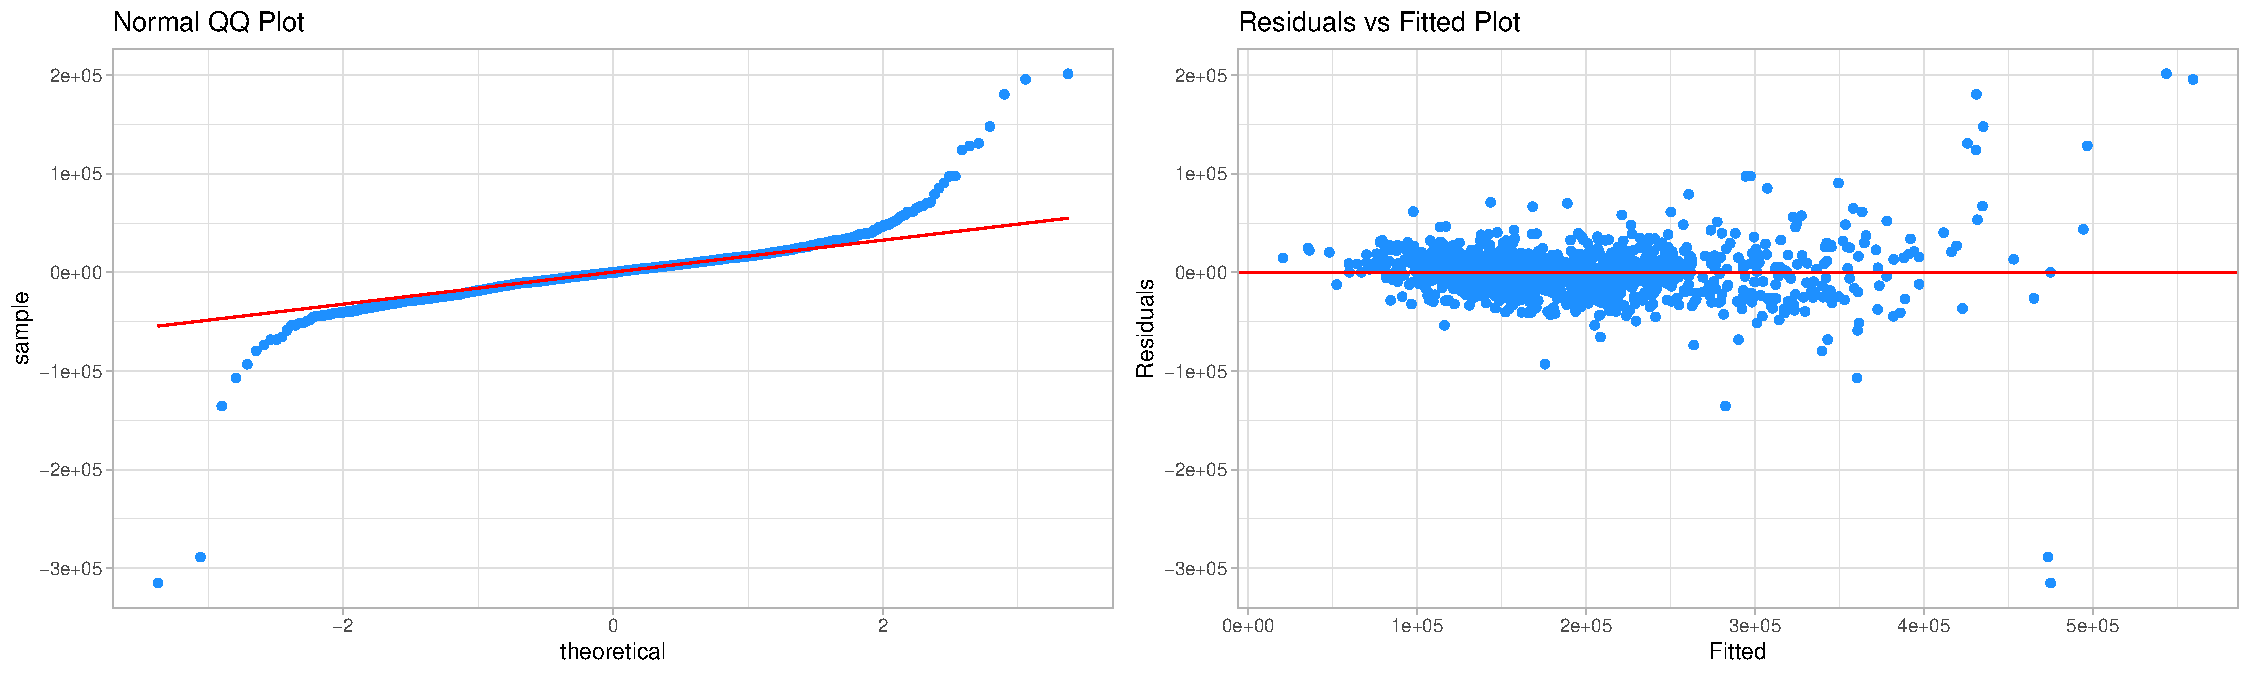
\includegraphics{Final-Project_files/figure-latex/unnamed-chunk-15-1.pdf}

\begin{verbatim}
## $num_predictors
## [1] 62
## 
## $shapiro_Normalcy_test_pvalue
## [1] 2.370924e-39
## 
## $bptest_Const_Variance_test_pvalue
## [1] 1.86925e-58
## 
## $RMSE
## [1] 26157.17
## 
## $AdjustedR2
## [1] 0.8707083
## 
## $AIC
## [1] 27621.95
\end{verbatim}

Based on the diagnostics we see that some kind of transformation for the response is necessary.

\hypertarget{boxcox-lambda-identifications-for-response-and-predictors}{%
\subsubsection{Boxcox lambda identifications for response and predictors}\label{boxcox-lambda-identifications-for-response-and-predictors}}

In order to figure out the transformation we find the lambda for it

\begin{Shaded}
\begin{Highlighting}[]
\KeywordTok{boxcox}\NormalTok{(m1)}
\end{Highlighting}
\end{Shaded}

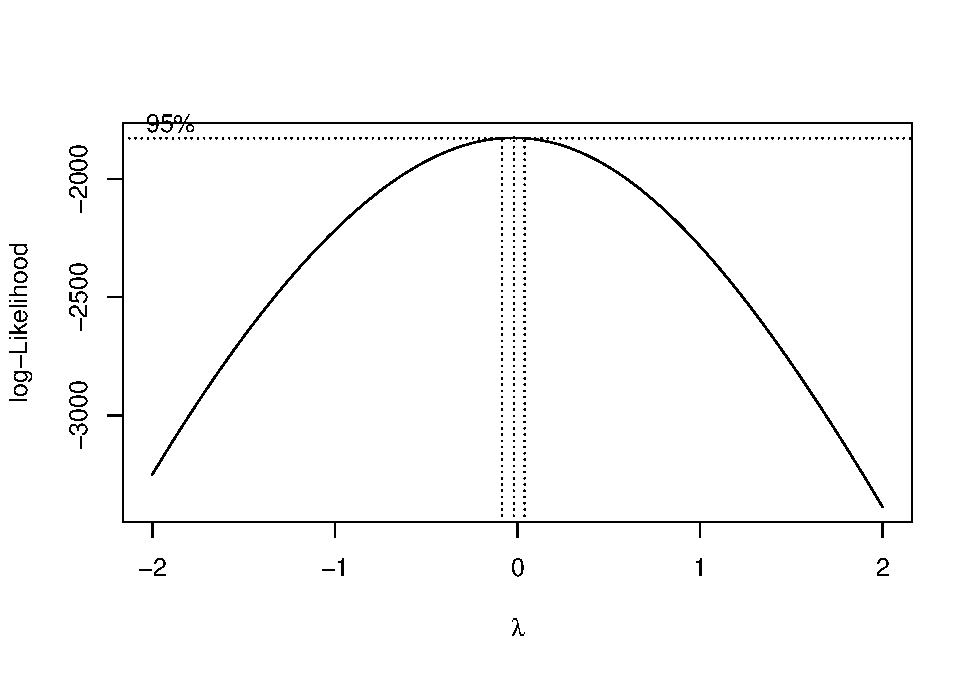
\includegraphics{Final-Project_files/figure-latex/unnamed-chunk-16-1.pdf}
We know that the most common Box-Cox Transformations are

\begin{longtable}[]{@{}ll@{}}
\toprule
\(\lambda\) & Tranasformed Data\tabularnewline
\midrule
\endhead
-2 & \(y^{-2}\)\tabularnewline
-1 & \(y^{-1}\)\tabularnewline
-.5 & \(1 \over \sqrt y\)\tabularnewline
0 & ln(y)\tabularnewline
.5 & \(\sqrt y\)\tabularnewline
1 & y\tabularnewline
2 & \(y^2\)\tabularnewline
\bottomrule
\end{longtable}

since our \(\lambda\) is close to 0 we will do log transformations

We redo the model and look at the diagnostics plots again

\begin{Shaded}
\begin{Highlighting}[]
\NormalTok{m2 <-}\StringTok{ }\KeywordTok{lm}\NormalTok{(}\StringTok{"log(SalePrice)~."}\NormalTok{, }\DataTypeTok{data=}\NormalTok{df_cols_removed)}
\KeywordTok{diagnostics}\NormalTok{(m2)}
\end{Highlighting}
\end{Shaded}

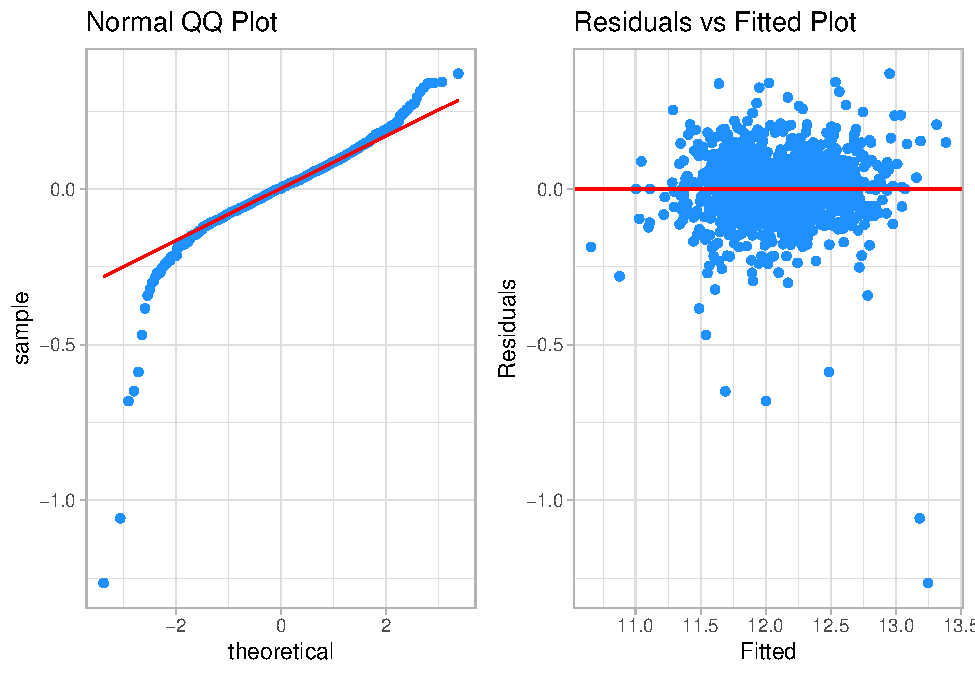
\includegraphics{Final-Project_files/figure-latex/unnamed-chunk-17-1.pdf}

\begin{verbatim}
## $num_predictors
## [1] 62
## 
## $shapiro_Normalcy_test_pvalue
## [1] 1.455201e-32
## 
## $bptest_Const_Variance_test_pvalue
## [1] 3.826722e-44
## 
## $RMSE
## [1] 0.1071
## 
## $AdjustedR2
## [1] 0.9049996
## 
## $AIC
## [1] -5576.829
\end{verbatim}

We see that the plots are a lot better, but there seems to be some scope for improvement.

Let us now identify the lamda transformations for the other columns we identified and using those variables as response, fit the model, but keep log(SalePrice) in the predictor with others

\begin{Shaded}
\begin{Highlighting}[]
\NormalTok{m3 <-}\StringTok{ }\KeywordTok{lm}\NormalTok{(}\StringTok{"LotArea~.-SalePrice+log(SalePrice)"}\NormalTok{, }\DataTypeTok{data =}\NormalTok{ df_cols_removed)}
\KeywordTok{boxcox}\NormalTok{(m3,}\DataTypeTok{xlab =} \StringTok{"lambda for LotArea"}\NormalTok{)}
\end{Highlighting}
\end{Shaded}

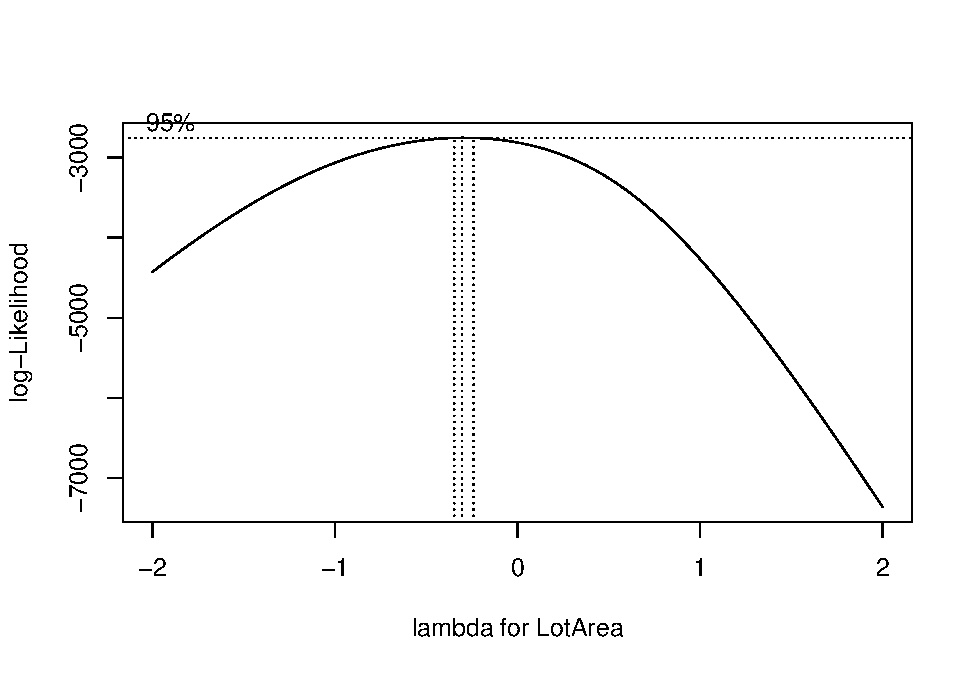
\includegraphics{Final-Project_files/figure-latex/unnamed-chunk-18-1.pdf}

We should apply log transformation to LotArea since \(\lambda\) is close to 0

\begin{Shaded}
\begin{Highlighting}[]
\NormalTok{m3 <-}\StringTok{ }\KeywordTok{lm}\NormalTok{(}\StringTok{"X1stFlrSF~.-SalePrice+log(SalePrice)"}\NormalTok{, }\DataTypeTok{data =}\NormalTok{ df_cols_removed)}
\KeywordTok{boxcox}\NormalTok{(m3,}\DataTypeTok{xlab =} \StringTok{"lambda for X1stFlrSF"}\NormalTok{)}
\end{Highlighting}
\end{Shaded}

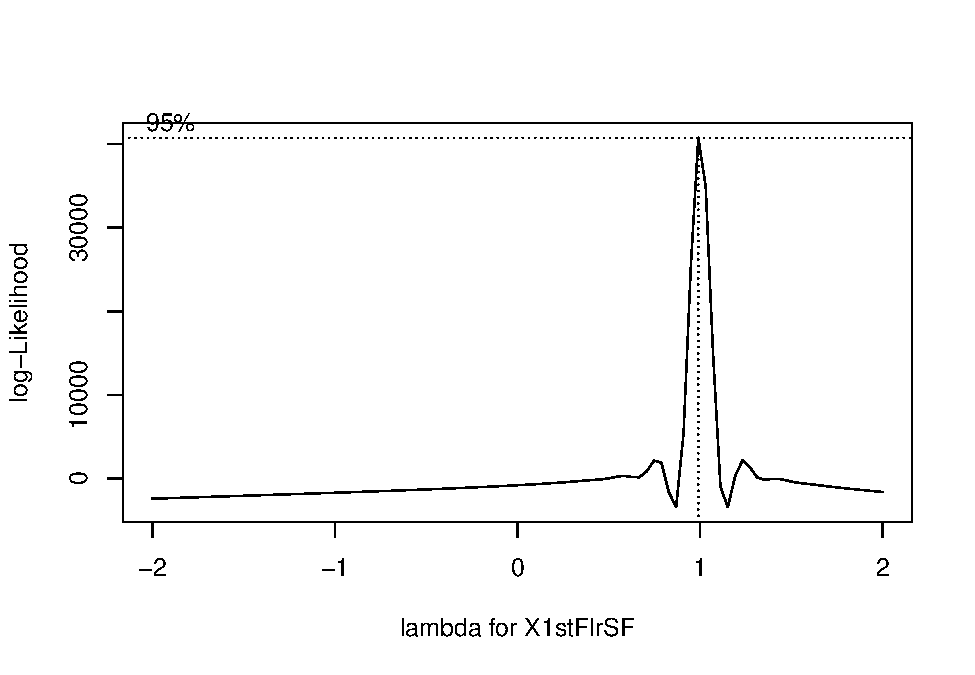
\includegraphics{Final-Project_files/figure-latex/unnamed-chunk-19-1.pdf}

There is no need to apply any transformation to X1stFlrSF

\begin{Shaded}
\begin{Highlighting}[]
\NormalTok{m3 <-}\StringTok{ }\KeywordTok{lm}\NormalTok{(}\StringTok{"GrLivArea~.-SalePrice+log(SalePrice)"}\NormalTok{, }\DataTypeTok{data =}\NormalTok{ df_cols_removed)}
\KeywordTok{boxcox}\NormalTok{(m3,}\DataTypeTok{xlab =} \StringTok{"lambda for GrLivArea"}\NormalTok{)}
\end{Highlighting}
\end{Shaded}

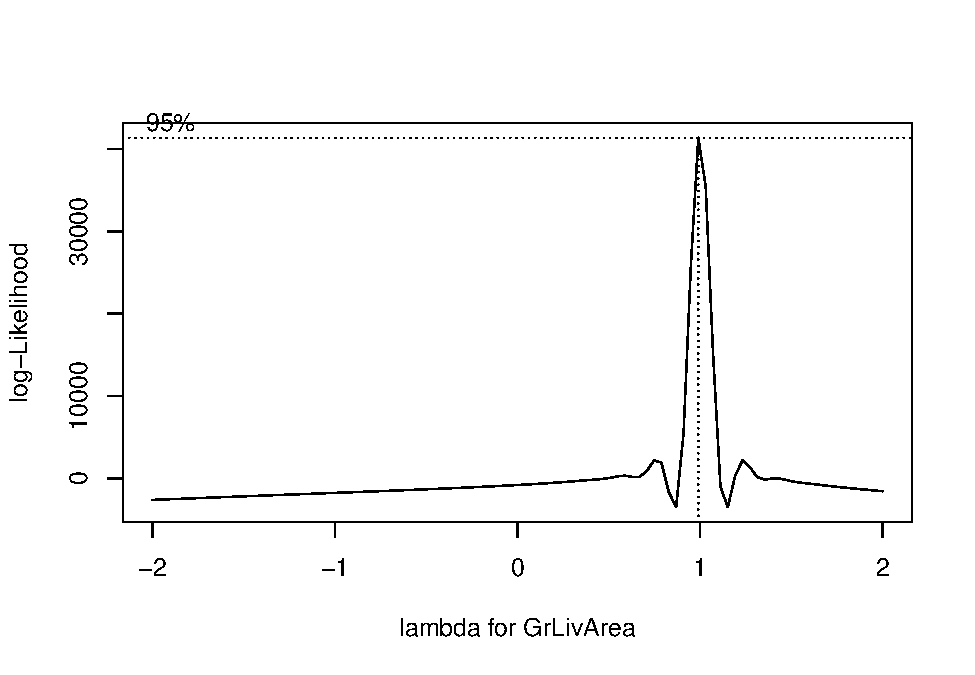
\includegraphics{Final-Project_files/figure-latex/unnamed-chunk-20-1.pdf}

There is no need to apply any transformation to GrLivArea

\begin{Shaded}
\begin{Highlighting}[]
\NormalTok{m3 <-}\StringTok{ }\KeywordTok{lm}\NormalTok{(}\StringTok{"GarageArea~.-SalePrice+log(SalePrice)"}\NormalTok{, }\DataTypeTok{data =}\NormalTok{ df_cols_removed)}
\KeywordTok{boxcox}\NormalTok{(m3,}\DataTypeTok{xlab =} \StringTok{"lambda for GarageArea"}\NormalTok{)}
\end{Highlighting}
\end{Shaded}

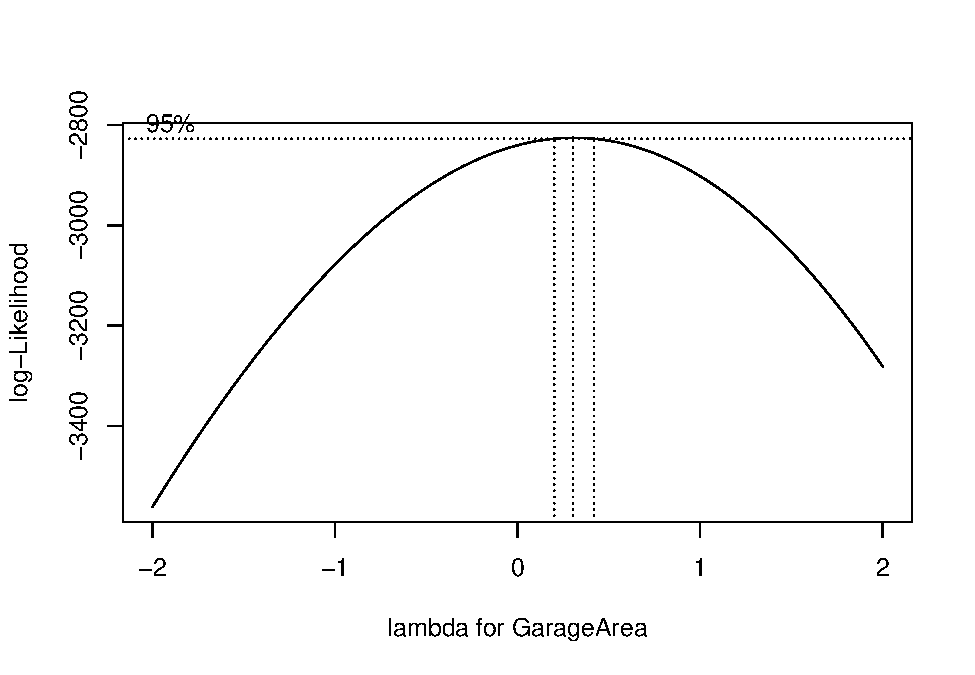
\includegraphics{Final-Project_files/figure-latex/unnamed-chunk-21-1.pdf}

We should apply log transformation to GarageArea since \(\lambda\) is close to 0

\begin{Shaded}
\begin{Highlighting}[]
\NormalTok{m3 <-}\StringTok{ }\KeywordTok{lm}\NormalTok{(}\StringTok{"YearBuilt~.-SalePrice+log(SalePrice)"}\NormalTok{, }\DataTypeTok{data =}\NormalTok{ df_cols_removed)}
\NormalTok{bc <-}\StringTok{ }\KeywordTok{boxcox}\NormalTok{(m3,}\DataTypeTok{xlab =} \StringTok{"lambda for YearBuilt"}\NormalTok{, }\DataTypeTok{lambda =} \KeywordTok{seq}\NormalTok{(}\OperatorTok{-}\DecValTok{200}\NormalTok{,}\DecValTok{400}\NormalTok{))}
\end{Highlighting}
\end{Shaded}

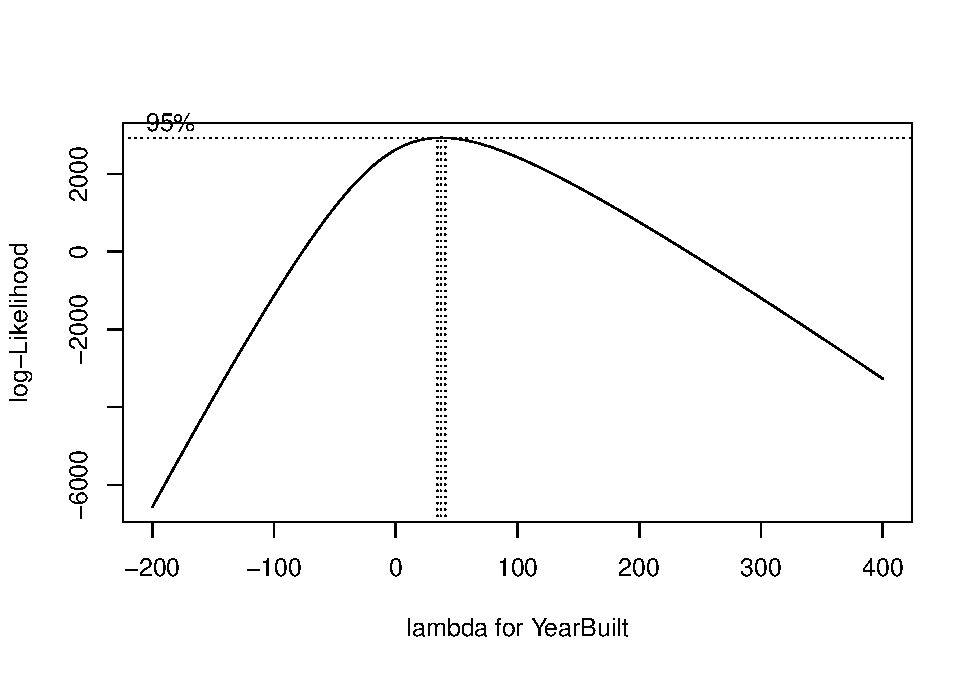
\includegraphics{Final-Project_files/figure-latex/unnamed-chunk-22-1.pdf}

\begin{Shaded}
\begin{Highlighting}[]
\NormalTok{(best_lam <-}\StringTok{ }\NormalTok{bc}\OperatorTok{$}\NormalTok{x[}\KeywordTok{which}\NormalTok{(bc}\OperatorTok{$}\NormalTok{y}\OperatorTok{==}\KeywordTok{max}\NormalTok{(bc}\OperatorTok{$}\NormalTok{y))])}
\end{Highlighting}
\end{Shaded}

\begin{verbatim}
## [1] 37
\end{verbatim}

\begin{Shaded}
\begin{Highlighting}[]
\NormalTok{m3 <-}\StringTok{ }\KeywordTok{lm}\NormalTok{(}\StringTok{"YearRemodAdd~.-SalePrice+log(SalePrice)"}\NormalTok{, }\DataTypeTok{data =}\NormalTok{ df_cols_removed)}
\NormalTok{bc <-}\StringTok{ }\KeywordTok{boxcox}\NormalTok{(m3,}\DataTypeTok{xlab =} \StringTok{"lambda for YearRemodAdd"}\NormalTok{, }\DataTypeTok{lambda =} \KeywordTok{seq}\NormalTok{(}\OperatorTok{-}\DecValTok{200}\NormalTok{,}\DecValTok{400}\NormalTok{))}
\end{Highlighting}
\end{Shaded}

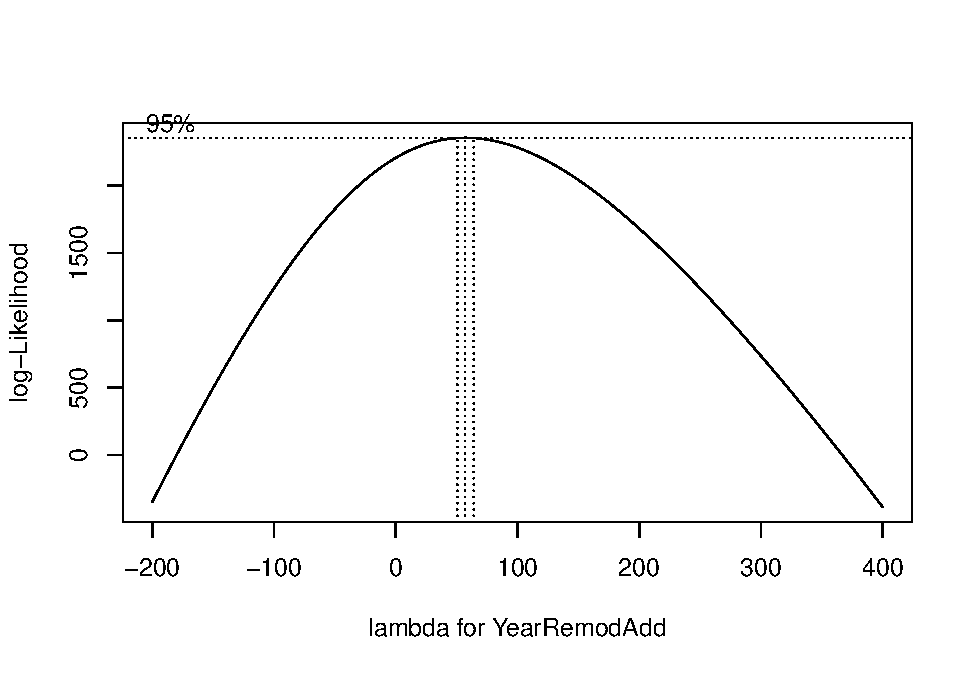
\includegraphics{Final-Project_files/figure-latex/unnamed-chunk-23-1.pdf}

\begin{Shaded}
\begin{Highlighting}[]
\NormalTok{(best_lam <-}\StringTok{ }\NormalTok{bc}\OperatorTok{$}\NormalTok{x[}\KeywordTok{which}\NormalTok{(bc}\OperatorTok{$}\NormalTok{y}\OperatorTok{==}\KeywordTok{max}\NormalTok{(bc}\OperatorTok{$}\NormalTok{y))])}
\end{Highlighting}
\end{Shaded}

\begin{verbatim}
## [1] 57
\end{verbatim}

YearBuilt and YearRemodAdd have very high \(\lambda\) and using these transformations will make it very hard to explain the model. We will keep a note of these two, and experiment with them if necessary

We will not identify the Lambda for MasVnrArea, BsmtFinSF1, BsmtFinSF2, WoodDeckSF, OpenPorchSF, EnclosedPorch since those predictors contant 0's, and we cant run the boxcox funtion on them unless we handle the 0's. Since we have a lot of predictors, we will not message these 6 predictors.

\hypertarget{model-identification}{%
\subsection{Model Identification}\label{model-identification}}

\hypertarget{simple-transformation-and-their-step-identified-model-comparison}{%
\subsubsection{Simple, transformation and their step identified model comparison}\label{simple-transformation-and-their-step-identified-model-comparison}}

Based on the above analysis we create the below models to start with

\begin{enumerate}
\def\labelenumi{\arabic{enumi})}
\tightlist
\item
  A simple additive model
\item
  A model with the above transformations but without the extreme transformations for YearBuilt and YearRemodAdd
\end{enumerate}

\begin{Shaded}
\begin{Highlighting}[]
\NormalTok{m_additive <-}\StringTok{ }\KeywordTok{lm}\NormalTok{(}\StringTok{"SalePrice~."}\NormalTok{, }\DataTypeTok{data =}\NormalTok{ df_cols_removed)}
\end{Highlighting}
\end{Shaded}

\begin{Shaded}
\begin{Highlighting}[]
\NormalTok{frm <-}\StringTok{ }\KeywordTok{create_formula}\NormalTok{(df_cols_removed, }\StringTok{"log(SalePrice)"}\NormalTok{, }\KeywordTok{c}\NormalTok{(}\StringTok{"SalePrice"}\NormalTok{, }\StringTok{"LotArea"}\NormalTok{, }\StringTok{"GarageArea"}\NormalTok{), }\KeywordTok{c}\NormalTok{(}\StringTok{"log(LotArea)"}\NormalTok{, }\StringTok{"log(GarageArea)"}\NormalTok{))}

\NormalTok{m_transform_}\DecValTok{1}\NormalTok{ <-}\StringTok{ }\KeywordTok{lm}\NormalTok{(}\DataTypeTok{formula =}\NormalTok{ frm, }\DataTypeTok{data =}\NormalTok{ df_cols_removed)}
\end{Highlighting}
\end{Shaded}

Now we use step backwards with aic for the above to find better versions of these models that are smaller than them

\begin{Shaded}
\begin{Highlighting}[]
\NormalTok{m_additive_step <-}\StringTok{ }\KeywordTok{step}\NormalTok{(m_additive, }\DataTypeTok{trace =} \DecValTok{0}\NormalTok{)}
\NormalTok{(frm <-}\StringTok{ }\KeywordTok{formula}\NormalTok{(m_additive_step))}
\end{Highlighting}
\end{Shaded}

\begin{verbatim}
## SalePrice ~ MSSubClass + MSZoning + LotArea + LotShape + LandContour + 
##     LotConfig + LandSlope + Neighborhood + Condition1 + BldgType + 
##     HouseStyle + OverallQual + OverallCond + YearBuilt + Exterior1st + 
##     MasVnrArea + ExterQual + BsmtQual + BsmtExposure + BsmtFinType1 + 
##     X1stFlrSF + X2ndFlrSF + LowQualFinSF + BsmtFullBath + FullBath + 
##     HalfBath + KitchenAbvGr + KitchenQual + Functional + Fireplaces + 
##     GarageArea + GarageQual + GarageCond + WoodDeckSF + OpenPorchSF + 
##     ScreenPorch + SaleCondition
## <environment: 0x0000000028da49a8>
\end{verbatim}

\begin{Shaded}
\begin{Highlighting}[]
\NormalTok{m_transform_}\DecValTok{1}\NormalTok{_step <-}\StringTok{ }\KeywordTok{step}\NormalTok{(m_transform_}\DecValTok{1}\NormalTok{, }\DataTypeTok{trace =} \DecValTok{0}\NormalTok{)}
\NormalTok{(frm <-}\StringTok{ }\KeywordTok{formula}\NormalTok{(m_transform_}\DecValTok{1}\NormalTok{_step))}
\end{Highlighting}
\end{Shaded}

\begin{verbatim}
## log(SalePrice) ~ MSSubClass + MSZoning + LotShape + LandContour + 
##     LotConfig + LandSlope + Neighborhood + Condition1 + OverallQual + 
##     OverallCond + YearBuilt + YearRemodAdd + Exterior1st + ExterCond + 
##     Foundation + BsmtQual + BsmtExposure + BsmtFinType1 + Heating + 
##     HeatingQC + CentralAir + X1stFlrSF + X2ndFlrSF + BsmtFullBath + 
##     FullBath + HalfBath + BedroomAbvGr + KitchenAbvGr + KitchenQual + 
##     Functional + Fireplaces + GarageQual + GarageCond + PavedDrive + 
##     WoodDeckSF + EnclosedPorch + ScreenPorch + SaleType + SaleCondition + 
##     log(LotArea) + log(GarageArea)
## <environment: 0x00000000207fac48>
\end{verbatim}

\begin{Shaded}
\begin{Highlighting}[]
\NormalTok{m_additive_result <-}\StringTok{ }\KeywordTok{diagnostics}\NormalTok{(m_additive, }\DataTypeTok{plotit =} \OtherTok{FALSE}\NormalTok{)}
\NormalTok{m_additive_step_result <-}\StringTok{ }\KeywordTok{diagnostics}\NormalTok{(m_additive_step, }\DataTypeTok{plotit =} \OtherTok{FALSE}\NormalTok{)}

\NormalTok{m_transform_}\DecValTok{1}\NormalTok{_result <-}\StringTok{ }\KeywordTok{diagnostics}\NormalTok{(m_transform_}\DecValTok{1}\NormalTok{, }\DataTypeTok{plotit =} \OtherTok{FALSE}\NormalTok{)}
\NormalTok{m_transform_}\DecValTok{1}\NormalTok{_step_result <-}\StringTok{ }\KeywordTok{diagnostics}\NormalTok{(m_transform_}\DecValTok{1}\NormalTok{_step, }\DataTypeTok{plotit =} \OtherTok{FALSE}\NormalTok{)}

\NormalTok{df_result <-}\StringTok{ }\KeywordTok{rbind}\NormalTok{(}\DataTypeTok{m_additive =}\NormalTok{ m_additive_result, }
                   \DataTypeTok{m_additive_step =}\NormalTok{ m_additive_step_result, }
                   \DataTypeTok{m_transform_1 =}\NormalTok{ m_transform_}\DecValTok{1}\NormalTok{_result, }
                   \DataTypeTok{m_transform_1_step =}\NormalTok{ m_transform_}\DecValTok{1}\NormalTok{_step_result)}

\NormalTok{knitr}\OperatorTok{::}\KeywordTok{kable}\NormalTok{(df_result)}
\end{Highlighting}
\end{Shaded}

\begin{tabular}{l|l|l|l|l|l|l}
\hline
  & num\_predictors & shapiro\_Normalcy\_test\_pvalue & bptest\_Const\_Variance\_test\_pvalue & RMSE & AdjustedR2 & AIC\\
\hline
m\_additive & 62 & 2.37092379058517e-39 & 1.86925015440473e-58 & 26157.1698 & 0.870708279573272 & 27621.9471671102\\
\hline
m\_additive\_step & 37 & 5.07711813649292e-40 & 8.93991489455308e-57 & 26813.2929 & 0.872442547569793 & 27540.2435555701\\
\hline
m\_transform\_1 & 62 & 6.52432665283327e-33 & 7.1310972543544e-43 & 0.1059 & 0.907079883830508 & -5606.45451163626\\
\hline
m\_transform\_1\_step & 41 & 2.58532434377342e-34 & 1.56280913290727e-38 & 0.1085 & 0.907631103431557 & -5668.25929379707\\
\hline
\end{tabular}

Looking at the above table, we can clearly see that the additive model isnt yielding a good model. The RMSE is extremely high. Hence we will discard this model for now.

\hypertarget{anova-test}{%
\subsubsection{Anova test}\label{anova-test}}

In order to confirm that this is a better model of the two, we will do anova test

\begin{Shaded}
\begin{Highlighting}[]
\KeywordTok{anova}\NormalTok{(m_transform_}\DecValTok{1}\NormalTok{, m_transform_}\DecValTok{1}\NormalTok{_step)}
\end{Highlighting}
\end{Shaded}

\begin{verbatim}
## Analysis of Variance Table
## 
## Model 1: log(SalePrice) ~ MSSubClass + MSZoning + LotShape + LandContour + 
##     LotConfig + LandSlope + Neighborhood + Condition1 + BldgType + 
##     HouseStyle + OverallQual + OverallCond + YearBuilt + YearRemodAdd + 
##     RoofStyle + Exterior1st + Exterior2nd + MasVnrType + MasVnrArea + 
##     ExterQual + ExterCond + Foundation + BsmtQual + BsmtCond + 
##     BsmtExposure + BsmtFinType1 + BsmtFinSF1 + BsmtFinType2 + 
##     BsmtFinSF2 + BsmtUnfSF + Heating + HeatingQC + CentralAir + 
##     Electrical + X1stFlrSF + X2ndFlrSF + LowQualFinSF + GrLivArea + 
##     BsmtFullBath + BsmtHalfBath + FullBath + HalfBath + BedroomAbvGr + 
##     KitchenAbvGr + KitchenQual + Functional + Fireplaces + GarageType + 
##     GarageFinish + GarageQual + GarageCond + PavedDrive + WoodDeckSF + 
##     OpenPorchSF + EnclosedPorch + ScreenPorch + MoSold + YrSold + 
##     SaleType + SaleCondition + log(LotArea) + log(GarageArea)
## Model 2: log(SalePrice) ~ MSSubClass + MSZoning + LotShape + LandContour + 
##     LotConfig + LandSlope + Neighborhood + Condition1 + OverallQual + 
##     OverallCond + YearBuilt + YearRemodAdd + Exterior1st + ExterCond + 
##     Foundation + BsmtQual + BsmtExposure + BsmtFinType1 + Heating + 
##     HeatingQC + CentralAir + X1stFlrSF + X2ndFlrSF + BsmtFullBath + 
##     FullBath + HalfBath + BedroomAbvGr + KitchenAbvGr + KitchenQual + 
##     Functional + Fireplaces + GarageQual + GarageCond + PavedDrive + 
##     WoodDeckSF + EnclosedPorch + ScreenPorch + SaleType + SaleCondition + 
##     log(LotArea) + log(GarageArea)
##   Res.Df    RSS  Df Sum of Sq     F Pr(>F)
## 1   1137 15.004                           
## 2   1200 15.741 -63  -0.73741 0.887 0.7218
\end{verbatim}

Based on the anova test, we see that the smaller model is sufficient hence we move ahead with m\_transform\_1

Hence we will use m\_transform\_1\_step model going forward

\begin{Shaded}
\begin{Highlighting}[]
\KeywordTok{formula}\NormalTok{(m_transform_}\DecValTok{1}\NormalTok{_step)}
\end{Highlighting}
\end{Shaded}

\begin{verbatim}
## log(SalePrice) ~ MSSubClass + MSZoning + LotShape + LandContour + 
##     LotConfig + LandSlope + Neighborhood + Condition1 + OverallQual + 
##     OverallCond + YearBuilt + YearRemodAdd + Exterior1st + ExterCond + 
##     Foundation + BsmtQual + BsmtExposure + BsmtFinType1 + Heating + 
##     HeatingQC + CentralAir + X1stFlrSF + X2ndFlrSF + BsmtFullBath + 
##     FullBath + HalfBath + BedroomAbvGr + KitchenAbvGr + KitchenQual + 
##     Functional + Fireplaces + GarageQual + GarageCond + PavedDrive + 
##     WoodDeckSF + EnclosedPorch + ScreenPorch + SaleType + SaleCondition + 
##     log(LotArea) + log(GarageArea)
## <environment: 0x00000000207fac48>
\end{verbatim}

\hypertarget{individual-parameter-significance-test}{%
\subsubsection{Individual parameter significance test}\label{individual-parameter-significance-test}}

Looking at the diagnostics, our model can still do better. We will now look at the individual significant of the parameters of this model to see if we can eliminate any predictors

\begin{Shaded}
\begin{Highlighting}[]
\NormalTok{a <-}\StringTok{ }\KeywordTok{coef}\NormalTok{(}\KeywordTok{summary}\NormalTok{(m_transform_}\DecValTok{1}\NormalTok{_step))[,}\StringTok{"Pr(>|t|)"}\NormalTok{] }
\KeywordTok{names}\NormalTok{(a)}
\end{Highlighting}
\end{Shaded}

\begin{verbatim}
##   [1] "(Intercept)"          "MSSubClass"           "MSZoningFV"          
##   [4] "MSZoningRH"           "MSZoningRL"           "MSZoningRM"          
##   [7] "LotShapeIR2"          "LotShapeIR3"          "LotShapeReg"         
##  [10] "LandContourHLS"       "LandContourLow"       "LandContourLvl"      
##  [13] "LotConfigCulDSac"     "LotConfigFR2"         "LotConfigFR3"        
##  [16] "LotConfigInside"      "LandSlopeMod"         "LandSlopeSev"        
##  [19] "NeighborhoodBlueste"  "NeighborhoodBrDale"   "NeighborhoodBrkSide" 
##  [22] "NeighborhoodClearCr"  "NeighborhoodCollgCr"  "NeighborhoodCrawfor" 
##  [25] "NeighborhoodEdwards"  "NeighborhoodGilbert"  "NeighborhoodIDOTRR"  
##  [28] "NeighborhoodMeadowV"  "NeighborhoodMitchel"  "NeighborhoodNAmes"   
##  [31] "NeighborhoodNoRidge"  "NeighborhoodNPkVill"  "NeighborhoodNridgHt" 
##  [34] "NeighborhoodNWAmes"   "NeighborhoodOldTown"  "NeighborhoodSawyer"  
##  [37] "NeighborhoodSawyerW"  "NeighborhoodSomerst"  "NeighborhoodStoneBr" 
##  [40] "NeighborhoodSWISU"    "NeighborhoodTimber"   "NeighborhoodVeenker" 
##  [43] "Condition1Feedr"      "Condition1Norm"       "Condition1PosA"      
##  [46] "Condition1PosN"       "Condition1RRAe"       "Condition1RRAn"      
##  [49] "Condition1RRNe"       "Condition1RRNn"       "OverallQual"         
##  [52] "OverallCond"          "YearBuilt"            "YearRemodAdd"        
##  [55] "Exterior1stBrkComm"   "Exterior1stBrkFace"   "Exterior1stCBlock"   
##  [58] "Exterior1stCemntBd"   "Exterior1stHdBoard"   "Exterior1stImStucc"  
##  [61] "Exterior1stMetalSd"   "Exterior1stPlywood"   "Exterior1stStone"    
##  [64] "Exterior1stStucco"    "Exterior1stVinylSd"   "Exterior1stWd Sdng"  
##  [67] "Exterior1stWdShing"   "ExterCondFa"          "ExterCondGd"         
##  [70] "ExterCondTA"          "FoundationCBlock"     "FoundationPConc"     
##  [73] "FoundationStone"      "FoundationWood"       "BsmtQualFa"          
##  [76] "BsmtQualGd"           "BsmtQualTA"           "BsmtExposureGd"      
##  [79] "BsmtExposureMn"       "BsmtExposureNo"       "BsmtFinType1BLQ"     
##  [82] "BsmtFinType1GLQ"      "BsmtFinType1LwQ"      "BsmtFinType1Rec"     
##  [85] "BsmtFinType1Unf"      "HeatingGasW"          "HeatingGrav"         
##  [88] "HeatingOthW"          "HeatingQCFa"          "HeatingQCGd"         
##  [91] "HeatingQCPo"          "HeatingQCTA"          "CentralAirY"         
##  [94] "X1stFlrSF"            "X2ndFlrSF"            "BsmtFullBath"        
##  [97] "FullBath"             "HalfBath"             "BedroomAbvGr"        
## [100] "KitchenAbvGr"         "KitchenQualFa"        "KitchenQualGd"       
## [103] "KitchenQualTA"        "FunctionalMaj2"       "FunctionalMin1"      
## [106] "FunctionalMin2"       "FunctionalMod"        "FunctionalSev"       
## [109] "FunctionalTyp"        "Fireplaces"           "GarageQualFa"        
## [112] "GarageQualGd"         "GarageQualPo"         "GarageQualTA"        
## [115] "GarageCondFa"         "GarageCondGd"         "GarageCondPo"        
## [118] "GarageCondTA"         "PavedDriveP"          "PavedDriveY"         
## [121] "WoodDeckSF"           "EnclosedPorch"        "ScreenPorch"         
## [124] "SaleTypeCon"          "SaleTypeConLD"        "SaleTypeConLI"       
## [127] "SaleTypeConLw"        "SaleTypeCWD"          "SaleTypeNew"         
## [130] "SaleTypeOth"          "SaleTypeWD"           "SaleConditionAdjLand"
## [133] "SaleConditionAlloca"  "SaleConditionFamily"  "SaleConditionNormal" 
## [136] "SaleConditionPartial" "log(LotArea)"         "log(GarageArea)"
\end{verbatim}

The above are all the coefficients of the model. We will use them to compare to the below filtered list of value \textgreater{} .1

We will be conservative and use alpha = .1 We now identify the individual columns that have p-value of greater than .1 and remove them from the dataset to create another model

\begin{Shaded}
\begin{Highlighting}[]
\KeywordTok{names}\NormalTok{(a[a}\OperatorTok{>}\NormalTok{.}\DecValTok{01}\NormalTok{])}
\end{Highlighting}
\end{Shaded}

\begin{verbatim}
##  [1] "LotShapeIR2"          "LotShapeReg"          "LandContourLow"      
##  [4] "LotConfigCulDSac"     "LotConfigFR2"         "LotConfigFR3"        
##  [7] "LotConfigInside"      "LandSlopeMod"         "LandSlopeSev"        
## [10] "NeighborhoodBlueste"  "NeighborhoodBrDale"   "NeighborhoodBrkSide" 
## [13] "NeighborhoodClearCr"  "NeighborhoodCollgCr"  "NeighborhoodCrawfor" 
## [16] "NeighborhoodGilbert"  "NeighborhoodIDOTRR"   "NeighborhoodMitchel" 
## [19] "NeighborhoodNoRidge"  "NeighborhoodNPkVill"  "NeighborhoodNridgHt" 
## [22] "NeighborhoodNWAmes"   "NeighborhoodOldTown"  "NeighborhoodSawyer"  
## [25] "NeighborhoodSawyerW"  "NeighborhoodSomerst"  "NeighborhoodSWISU"   
## [28] "NeighborhoodTimber"   "NeighborhoodVeenker"  "Condition1Feedr"     
## [31] "Condition1PosA"       "Condition1PosN"       "Condition1RRAe"      
## [34] "Condition1RRAn"       "Condition1RRNe"       "Condition1RRNn"      
## [37] "YearRemodAdd"         "Exterior1stCBlock"    "Exterior1stCemntBd"  
## [40] "Exterior1stHdBoard"   "Exterior1stImStucc"   "Exterior1stMetalSd"  
## [43] "Exterior1stPlywood"   "Exterior1stStone"     "Exterior1stStucco"   
## [46] "Exterior1stVinylSd"   "Exterior1stWd Sdng"   "Exterior1stWdShing"  
## [49] "ExterCondFa"          "ExterCondGd"          "ExterCondTA"         
## [52] "FoundationCBlock"     "FoundationWood"       "BsmtQualFa"          
## [55] "BsmtExposureMn"       "BsmtExposureNo"       "BsmtFinType1BLQ"     
## [58] "BsmtFinType1GLQ"      "BsmtFinType1LwQ"      "BsmtFinType1Rec"     
## [61] "HeatingGrav"          "HeatingOthW"          "HeatingQCFa"         
## [64] "HeatingQCGd"          "HeatingQCPo"          "KitchenAbvGr"        
## [67] "FunctionalMin1"       "FunctionalMin2"       "FunctionalMod"       
## [70] "FunctionalSev"        "FunctionalTyp"        "PavedDriveP"         
## [73] "PavedDriveY"          "EnclosedPorch"        "SaleTypeCon"         
## [76] "SaleTypeConLD"        "SaleTypeConLI"        "SaleTypeConLw"       
## [79] "SaleTypeCWD"          "SaleTypeNew"          "SaleTypeOth"         
## [82] "SaleTypeWD"           "SaleConditionAdjLand" "SaleConditionAlloca" 
## [85] "SaleConditionFamily"  "SaleConditionPartial"
\end{verbatim}

We see that there are no variables that have p-value \textless{} .1, implying that all the variables have a significant relationship with the response

We will select all non-categorical variables that have \(pvalue>.1\) and will will choose only the categorical predictors to remove that have all of the categories with \(pvalue>.1\)

\begin{itemize}
\tightlist
\item
  LandSlope - Intutively we think this is important hence we will not remove it
\item
  YearRemodAdd
\item
  ExterCond
\item
  KitchenAbvGr - we intutively think this is important and will not remove it
\item
  PavedDrive
\item
  EnclosedPorch
\item
  SaleType - Intutively we think this is important hence we will not remove it
\end{itemize}

Now we modify the formula of the model that is best so far, m\_transform\_1, and remove the above 5 predictors from it

\begin{Shaded}
\begin{Highlighting}[]
\NormalTok{remove_cols3 <-}\StringTok{ }\KeywordTok{c}\NormalTok{(}\StringTok{"YearRemodAdd"}\NormalTok{,}\StringTok{"ExterCond"}\NormalTok{, }\StringTok{"PavedDrive"}\NormalTok{, }\StringTok{"EnclosedPorch"}\NormalTok{)}

\NormalTok{f <-}\StringTok{ }\KeywordTok{formula}\NormalTok{(m_transform_}\DecValTok{1}\NormalTok{_step)}
\NormalTok{predictor_list <-}\StringTok{ }\KeywordTok{str_split}\NormalTok{(f, }\DataTypeTok{pattern =} \KeywordTok{fixed}\NormalTok{(}\StringTok{" + "}\NormalTok{))[[}\DecValTok{3}\NormalTok{]]}
\NormalTok{predictor_list <-}\StringTok{ }\NormalTok{predictor_list[}\OperatorTok{!}\NormalTok{(predictor_list }\OperatorTok\StringTok{ }\NormalTok{remove_cols3)]}
\CommentTok{# replacing the \textbackslash{}n that str_spit introduces after 500 characters}
\NormalTok{predictor_list <-}\StringTok{ }\KeywordTok{str_replace}\NormalTok{(predictor_list, }\StringTok{"}\CharTok{\textbackslash{}n}\StringTok{    "}\NormalTok{, }\StringTok{""}\NormalTok{)}
\CommentTok{# create the formula}
\NormalTok{(frm1 <-}\StringTok{ }\KeywordTok{paste}\NormalTok{(}\StringTok{"log(SalePrice) ~ "}\NormalTok{, }\KeywordTok{paste}\NormalTok{(predictor_list, }\DataTypeTok{collapse =} \StringTok{' + '}\NormalTok{)))}
\end{Highlighting}
\end{Shaded}

\begin{verbatim}
## [1] "log(SalePrice) ~  MSSubClass + MSZoning + LotShape + LandContour + LotConfig + LandSlope + Neighborhood + Condition1 + OverallQual + OverallCond + YearBuilt + Exterior1st + Foundation + BsmtQual + BsmtExposure + BsmtFinType1 + Heating + HeatingQC + CentralAir + X1stFlrSF + X2ndFlrSF + BsmtFullBath + FullBath + HalfBath + BedroomAbvGr + KitchenAbvGr + KitchenQual + Functional + Fireplaces + GarageQual + GarageCond + WoodDeckSF + ScreenPorch + SaleType + SaleCondition + log(LotArea) + log(GarageArea)"
\end{verbatim}

Now we use the above formula to create the model and look at its diagnostics

\begin{Shaded}
\begin{Highlighting}[]
\NormalTok{m_transform_}\DecValTok{1}\NormalTok{_step_sig_only <-}\StringTok{ }\KeywordTok{lm}\NormalTok{(frm1, }\DataTypeTok{data =}\NormalTok{ df_cols_removed)}
\end{Highlighting}
\end{Shaded}

We do an anova test between the two models to make sure we have not discarded significant predictors

\begin{Shaded}
\begin{Highlighting}[]
\KeywordTok{anova}\NormalTok{(m_transform_}\DecValTok{1}\NormalTok{_step_sig_only, m_transform_}\DecValTok{1}\NormalTok{_step)}
\end{Highlighting}
\end{Shaded}

\begin{verbatim}
## Analysis of Variance Table
## 
## Model 1: log(SalePrice) ~ MSSubClass + MSZoning + LotShape + LandContour + 
##     LotConfig + LandSlope + Neighborhood + Condition1 + OverallQual + 
##     OverallCond + YearBuilt + Exterior1st + Foundation + BsmtQual + 
##     BsmtExposure + BsmtFinType1 + Heating + HeatingQC + CentralAir + 
##     X1stFlrSF + X2ndFlrSF + BsmtFullBath + FullBath + HalfBath + 
##     BedroomAbvGr + KitchenAbvGr + KitchenQual + Functional + 
##     Fireplaces + GarageQual + GarageCond + WoodDeckSF + ScreenPorch + 
##     SaleType + SaleCondition + log(LotArea) + log(GarageArea)
## Model 2: log(SalePrice) ~ MSSubClass + MSZoning + LotShape + LandContour + 
##     LotConfig + LandSlope + Neighborhood + Condition1 + OverallQual + 
##     OverallCond + YearBuilt + YearRemodAdd + Exterior1st + ExterCond + 
##     Foundation + BsmtQual + BsmtExposure + BsmtFinType1 + Heating + 
##     HeatingQC + CentralAir + X1stFlrSF + X2ndFlrSF + BsmtFullBath + 
##     FullBath + HalfBath + BedroomAbvGr + KitchenAbvGr + KitchenQual + 
##     Functional + Fireplaces + GarageQual + GarageCond + PavedDrive + 
##     WoodDeckSF + EnclosedPorch + ScreenPorch + SaleType + SaleCondition + 
##     log(LotArea) + log(GarageArea)
##   Res.Df    RSS Df Sum of Sq      F  Pr(>F)  
## 1   1207 15.984                              
## 2   1200 15.741  7   0.24236 2.6394 0.01039 *
## ---
## Signif. codes:  0 '***' 0.001 '**' 0.01 '*' 0.05 '.' 0.1 ' ' 1
\end{verbatim}

Based on the result of the anova test, we see that for our smaller model we fail to reject the Null Hypothesis, hence we move ahead with this model

Now we will compare the diagnostics of the 2 models

\begin{Shaded}
\begin{Highlighting}[]
\NormalTok{m_transform_}\DecValTok{1}\NormalTok{_step_result <-}\StringTok{ }\KeywordTok{diagnostics}\NormalTok{(m_transform_}\DecValTok{1}\NormalTok{_step, }\DataTypeTok{plotit =} \OtherTok{FALSE}\NormalTok{)}
\NormalTok{m_transform_}\DecValTok{1}\NormalTok{_step_sig_only_result <-}\StringTok{ }\KeywordTok{diagnostics}\NormalTok{(m_transform_}\DecValTok{1}\NormalTok{_step_sig_only, }\DataTypeTok{plotit =} \OtherTok{FALSE}\NormalTok{)}

\NormalTok{df_result <-}\StringTok{ }\KeywordTok{rbind}\NormalTok{(}\DataTypeTok{m_transform_1_step=}\NormalTok{m_transform_}\DecValTok{1}\NormalTok{_step_result, }\DataTypeTok{m_transform_1_step_sig_only=}\NormalTok{m_transform_}\DecValTok{1}\NormalTok{_step_sig_only_result)}

\NormalTok{knitr}\OperatorTok{::}\KeywordTok{kable}\NormalTok{(df_result)}
\end{Highlighting}
\end{Shaded}

\begin{tabular}{l|l|l|l|l|l|l}
\hline
  & num\_predictors & shapiro\_Normalcy\_test\_pvalue & bptest\_Const\_Variance\_test\_pvalue & RMSE & AdjustedR2 & AIC\\
\hline
m\_transform\_1\_step & 41 & 2.58532434377342e-34 & 1.56280913290727e-38 & 0.1085 & 0.907631103431557 & -5668.25929379707\\
\hline
m\_transform\_1\_step\_sig\_only & 37 & 4.37061579785164e-34 & 8.2169301822451e-41 & 0.1093 & 0.906752877081228 & -5661.81561020389\\
\hline
\end{tabular}

We see that our diagnostic statistics are about the same. Hence we will select the smaller model, m\_transform\_1\_step\_sig\_only, as our better model

\hypertarget{variance-inflation-factor-identification}{%
\subsubsection{Variance Inflation factor identification}\label{variance-inflation-factor-identification}}

We look at variance inflation factors, and filter by only vifs that are \textgreater5

\begin{Shaded}
\begin{Highlighting}[]
\NormalTok{faraway}\OperatorTok{::}\KeywordTok{vif}\NormalTok{(m_transform_}\DecValTok{1}\NormalTok{_step_sig_only)[faraway}\OperatorTok{::}\KeywordTok{vif}\NormalTok{(m_transform_}\DecValTok{1}\NormalTok{_step_sig_only)}\OperatorTok{>}\DecValTok{5}\NormalTok{]}
\end{Highlighting}
\end{Shaded}

\begin{verbatim}
##           MSZoningFV           MSZoningRL           MSZoningRM 
##            16.951121            46.304868            30.796731 
##  NeighborhoodBrkSide  NeighborhoodCollgCr  NeighborhoodCrawfor 
##             6.555110            11.190361             5.942716 
##  NeighborhoodEdwards  NeighborhoodGilbert   NeighborhoodIDOTRR 
##             7.019645             7.278823             5.593370 
##    NeighborhoodNAmes  NeighborhoodNridgHt   NeighborhoodNWAmes 
##            17.587236             6.332576             7.423773 
##  NeighborhoodOldTown   NeighborhoodSawyer  NeighborhoodSawyerW 
##            13.850877             7.276555             5.324532 
##  NeighborhoodSomerst            YearBuilt   Exterior1stCemntBd 
##            10.264811            12.185867             6.075455 
##   Exterior1stHdBoard   Exterior1stMetalSd   Exterior1stPlywood 
##            16.911965            15.568023             9.594118 
##   Exterior1stVinylSd   Exterior1stWd Sdng     FoundationCBlock 
##            28.365722            14.420805             7.164986 
##      FoundationPConc           BsmtQualGd           BsmtQualTA 
##             8.360265             6.207361             9.867833 
##            X2ndFlrSF        KitchenQualGd        KitchenQualTA 
##             5.579018             6.649901             8.842501 
##        FunctionalTyp         GarageQualFa         GarageQualGd 
##             9.189799            55.405873            17.197621 
##         GarageQualPo         GarageQualTA         GarageCondFa 
##             5.768295            75.730585            56.169150 
##         GarageCondGd         GarageCondPo         GarageCondTA 
##            16.322905            14.504310            83.417516 
##          SaleTypeNew           SaleTypeWD SaleConditionPartial 
##            46.188707             5.129151            44.139760
\end{verbatim}

We notice that while there are high vif values, they are for categorical variables, and hence we choose to do nothing with this. There is YearBuilt, but it is not large enough for us to remove it, and individually we have already seen above, that it seems to have a significant relationship with the response. Hence we make no changes

\hypertarget{influential-points-identification-and-handling}{%
\subsubsection{Influential points identification and handling}\label{influential-points-identification-and-handling}}

We will now look at high influence points and investigate them

\begin{Shaded}
\begin{Highlighting}[]
\NormalTok{influentials <-}\StringTok{ }\KeywordTok{which}\NormalTok{(}\KeywordTok{cooks.distance}\NormalTok{(m_transform_}\DecValTok{1}\NormalTok{_step_sig_only) }\OperatorTok{>}\StringTok{ }\NormalTok{(}\DecValTok{4} \OperatorTok{/}\StringTok{ }\KeywordTok{length}\NormalTok{(}\KeywordTok{cooks.distance}\NormalTok{(m_transform_}\DecValTok{1}\NormalTok{_step_sig_only))))}
\KeywordTok{length}\NormalTok{(influentials)}
\end{Highlighting}
\end{Shaded}

\begin{verbatim}
## [1] 95
\end{verbatim}

As an experiment we try and remove the influentials and see what impact this has on the diagnostics

\begin{Shaded}
\begin{Highlighting}[]
\NormalTok{df_wo_influentials <-}\StringTok{ }\NormalTok{df_cols_removed[}\OperatorTok{-}\NormalTok{influentials,]}
\NormalTok{df_only_influentials <-}\StringTok{ }\NormalTok{df_cols_removed[influentials,]}

\NormalTok{m_no_influentials <-}\StringTok{ }\KeywordTok{lm}\NormalTok{(}\KeywordTok{formula}\NormalTok{(m_transform_}\DecValTok{1}\NormalTok{_step_sig_only), }\DataTypeTok{data =}\NormalTok{ df_wo_influentials)}
\end{Highlighting}
\end{Shaded}

Now we compare the diagnostics data

\begin{Shaded}
\begin{Highlighting}[]
\NormalTok{m_transform_}\DecValTok{1}\NormalTok{_step_sig_only_result <-}\StringTok{ }\KeywordTok{diagnostics}\NormalTok{(m_transform_}\DecValTok{1}\NormalTok{_step_sig_only, }\DataTypeTok{plotit =} \OtherTok{FALSE}\NormalTok{)}
\NormalTok{m_no_influentials_result <-}\StringTok{ }\KeywordTok{diagnostics}\NormalTok{(m_no_influentials, }\DataTypeTok{plotit =} \OtherTok{FALSE}\NormalTok{)}

\NormalTok{df_result <-}\StringTok{ }\KeywordTok{rbind}\NormalTok{(}\DataTypeTok{m_transform_1_step_sig_only =}\NormalTok{ m_transform_}\DecValTok{1}\NormalTok{_step_sig_only_result, }
                   \DataTypeTok{m_no_influentials =}\NormalTok{ m_no_influentials_result)}

\NormalTok{knitr}\OperatorTok{::}\KeywordTok{kable}\NormalTok{(df_result)}
\end{Highlighting}
\end{Shaded}

\begin{tabular}{l|l|l|l|l|l|l}
\hline
  & num\_predictors & shapiro\_Normalcy\_test\_pvalue & bptest\_Const\_Variance\_test\_pvalue & RMSE & AdjustedR2 & AIC\\
\hline
m\_transform\_1\_step\_sig\_only & 37 & 4.37061579785164e-34 & 8.2169301822451e-41 & 0.1093 & 0.906752877081228 & -5661.81561020389\\
\hline
m\_no\_influentials & 37 & 0.00105949872525489 & 0.00497557312769214 & 0.0691 & 0.958804107246139 & -6389.94189323825\\
\hline
\end{tabular}

We see that our diagnostics have improved significantly. We will have to sacrifice about 7\% of the observations but the improvements in RMSE and Adjusted Rsquare are significant. Hence we will So now we know that it is the influential points that are causing our model to have less than ideal diagnostics.

\hypertarget{selected-model}{%
\subsubsection{Selected model}\label{selected-model}}

Hence now our good model is m\_no\_influentials and the dataset is df\_wo\_influentials

\begin{Shaded}
\begin{Highlighting}[]
\KeywordTok{formula}\NormalTok{(m_no_influentials)}
\end{Highlighting}
\end{Shaded}

\begin{verbatim}
## log(SalePrice) ~ MSSubClass + MSZoning + LotShape + LandContour + 
##     LotConfig + LandSlope + Neighborhood + Condition1 + OverallQual + 
##     OverallCond + YearBuilt + Exterior1st + Foundation + BsmtQual + 
##     BsmtExposure + BsmtFinType1 + Heating + HeatingQC + CentralAir + 
##     X1stFlrSF + X2ndFlrSF + BsmtFullBath + FullBath + HalfBath + 
##     BedroomAbvGr + KitchenAbvGr + KitchenQual + Functional + 
##     Fireplaces + GarageQual + GarageCond + WoodDeckSF + ScreenPorch + 
##     SaleType + SaleCondition + log(LotArea) + log(GarageArea)
## <environment: 0x000000001f9e14b8>
\end{verbatim}

\hypertarget{results}{%
\section{Results}\label{results}}

We have already seen this in various places but we will now compare the diagnostics of all the models that we have seen to see how we have progressed

\begin{Shaded}
\begin{Highlighting}[]
\NormalTok{df_result <-}\StringTok{ }\KeywordTok{rbind}\NormalTok{(}\DataTypeTok{m_additive =}\NormalTok{ m_additive_result,}
                   \DataTypeTok{m_additive_step =}\NormalTok{ m_additive_step_result,}
                   \DataTypeTok{m_transform_1 =}\NormalTok{ m_transform_}\DecValTok{1}\NormalTok{_result,}
                   \DataTypeTok{m_transform_1_step =}\NormalTok{ m_transform_}\DecValTok{1}\NormalTok{_step_result,}
                   \DataTypeTok{m_transform_1_step_sig_only =}\NormalTok{ m_transform_}\DecValTok{1}\NormalTok{_step_sig_only_result, }
                   \DataTypeTok{m_no_influentials =}\NormalTok{ m_no_influentials_result)}

\NormalTok{knitr}\OperatorTok{::}\KeywordTok{kable}\NormalTok{(df_result)}
\end{Highlighting}
\end{Shaded}

\begin{tabular}{l|l|l|l|l|l|l}
\hline
  & num\_predictors & shapiro\_Normalcy\_test\_pvalue & bptest\_Const\_Variance\_test\_pvalue & RMSE & AdjustedR2 & AIC\\
\hline
m\_additive & 62 & 2.37092379058517e-39 & 1.86925015440473e-58 & 26157.1698 & 0.870708279573272 & 27621.9471671102\\
\hline
m\_additive\_step & 37 & 5.07711813649292e-40 & 8.93991489455308e-57 & 26813.2929 & 0.872442547569793 & 27540.2435555701\\
\hline
m\_transform\_1 & 62 & 6.52432665283327e-33 & 7.1310972543544e-43 & 0.1059 & 0.907079883830508 & -5606.45451163626\\
\hline
m\_transform\_1\_step & 41 & 2.58532434377342e-34 & 1.56280913290727e-38 & 0.1085 & 0.907631103431557 & -5668.25929379707\\
\hline
m\_transform\_1\_step\_sig\_only & 37 & 4.37061579785164e-34 & 8.2169301822451e-41 & 0.1093 & 0.906752877081228 & -5661.81561020389\\
\hline
m\_no\_influentials & 37 & 0.00105949872525489 & 0.00497557312769214 & 0.0691 & 0.958804107246139 & -6389.94189323825\\
\hline
\end{tabular}

We also look at the diagnostics plot of our selected model

\begin{Shaded}
\begin{Highlighting}[]
\KeywordTok{diagnostics}\NormalTok{(m_no_influentials, }\DataTypeTok{testit =} \OtherTok{FALSE}\NormalTok{)}
\end{Highlighting}
\end{Shaded}

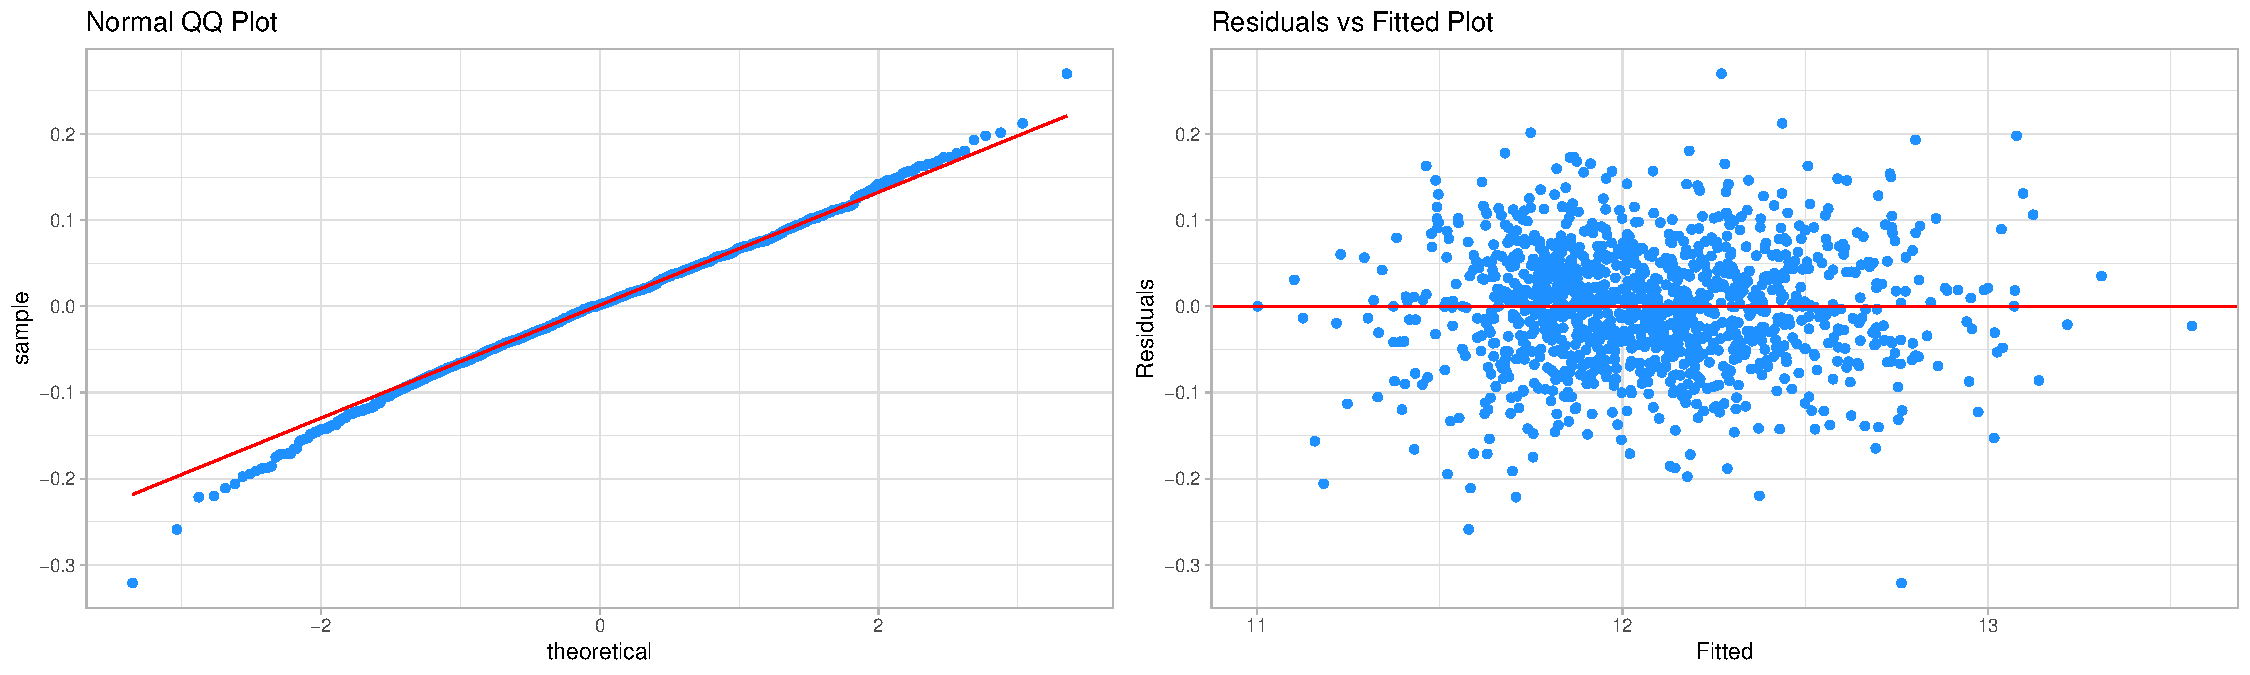
\includegraphics{Final-Project_files/figure-latex/unnamed-chunk-43-1.pdf}

Our diagnostics plots look fairly good We know that our shapiro test and BP test are rejecting the null hypothesis, but since the graphs looks pretty good, and we know that these tests are quick to reject for large datasets, we will select this model as our final model

\hypertarget{discussion}{%
\section{Discussion}\label{discussion}}

\hypertarget{result}{%
\section{Result}\label{result}}

\end{document}
